
\documentclass[onehalf,11pt]{beavtex}
\title{GPU-Based Fluid Structure Interaction using Immersed Boundary Methods}
\author{Christopher Minar}
\degree{Masters of Science}
\doctype{Masters Thesis}
\department{Mechanical Industrial and Manufacturing Engineering}
\depttype{School}
\depthead{Director}
\major{Mechanical Engineering}
\advisor{Kyle Niemeyer}
\submitdate{September 23, 2016}
\commencementyear{2016}
\abstract{Engineering applications often require fast, accurate solutions of fluid flow around freely moving bodies.
The massive parallelism enabled by GPU architecture enables high performance, offering a promising alternative to traditional solver acceleration via multicore CPUs.
However, fully harnessing GPU parallelism requires specialized algorithms and computing strategies.
This work modifies a direct-forcing immersed boundary method to model fluid-structure interaction and investigates its behavior on GPUs.
We performed verification of our solver using lid-driven cavity flow and impulsively started flow over a cylinder, and investigated its behavior with flow over a forced oscillating cylinder.}
\acknowledgements{We gratefully acknowledge the support of NVIDIA Corporation with the donation of the Tesla K\subsubsection0 GPU used for this research.
We also thank the Barba Group for developing, maintaining, and distributing their cuIBM code.}

\usepackage{algorithm}
\usepackage{algorithmic}
\usepackage[textsize=footnotesize]{todonotes}%used for inline todo notes with \todo[]{}
\usepackage{latexsym,amsmath,amssymb} %math packages
\usepackage{tikz} %used for tikz graphics
\usepackage{standalone}  %used for tikz graphics
\usetikzlibrary{shapes}  %used for tikz graphics
\usepackage{graphicx} %needed for subfigure
\usepackage{float,caption,subcaption} %figure stuff
\graphicspath{{./figure/}} %figure path
\usepackage{siunitx}
\sisetup{group-separator={,},
	detect-all,
	binary-units,
	list-units = single,
	range-units = single,
	tophrase = --,
	per-mode = symbol-or-fraction,
	separate-uncertainty = true,
	list-final-separator = {, and }
}


\begin{document}
\todo[inline]{fix margins}
\todo[inline]{change Fadlun to fadlun et al}
\maketitle

\mainmatter

\chapter{Introduction}
Immersed boundary methods (IBMs) are a broad term referring to of group of approaches used for simulating fluid flow over complex bodies.
The goal of IBMs is to represent a surface on a structured grid, removing the need to create a body fitted mesh.
These techniques are well-suited for simulating flow involving complex moving bodies because they do not require re-meshing between time steps.
We have developed an IBM solver for operation on graphics processing units (GPUs) designed to handle incompressible fluid--structure interaction problems with rigid bodies.

Peskin~\cite{Peskin:1972gh} first introduced the IBM in the 1970s to model blood flow with elastic boundaries.
The original IBM adds a forcing term to the Navier--Stokes equations that only acts near a body.
This forcing term simulates the force the body applies on the fluid, and is modeled as a spring.
Peskin's IBM was designed to handle elastic, deforming bodies.
One way to effectively implement Peskin's IBM for rigid bodies is to set a large spring coefficient; however, this makes the equations numerically stiff.

The IBM has since evolved to be applicable to a wide range of problems, as reviewed by Mittal and Iaccarino~\cite{Mittal:2005ii} and more recently Sotiropoulos and Yang~\cite{Sotiropoulos:2014gv}.
Mohd-Yusof~\cite{MohdYusof:1997wh} and Fadlun et al.~\cite{Fadlun:2000fl} developed a version for rigid bodies called the direct forcing method.
Instead of solving for the added force term in the Navier--Stokes equation, the velocities at the nodes nearest to the body are interpolated for using the body velocity to enforce the no-slip condition.
However, using the direct forcing method with a moving body causes numerical oscillations~\cite{liao2010simulating}~\cite{Luo:2012gx}.
This effect is manageable for preset motion but with a freely moving body the solver will poorly predict body position, velocity, and forces.
The numerical oscillations are caused by nodes switching representations between time steps, e.g., a node near the body (and thus treated differently) becoming a node solved for with the Navier--Stokes equations.
The approach of Luo et al.~\cite{Luo:2012gx} deals with the numerical oscillations by using a weighting function to transition between the two schemes.

The goal of this project is to develop a GPU-based solver capable of simulating 2D, incompressible flow over a moving, complex body. 
\todo[inline]{write end purpose of solver}
\todo[inline]{give solver a name}
\todo[inline]{add segment about lee and lee}
Chapter \ref{Numerical Methods} will discuss the theory of several direct forcing methods and their applicability to freely moving bodies. 
Chapter \ref{Implementation} cover the discretization of the methods as well as the challenges, strategies and implementation of the GPU.
Chapter \ref{Validation} will show the validation and verification of different aspects of the solver using five different test cases; lid driven cavity, flow over an impulsively started cylinder, forced motion of a cylinder in static flow, forced motion of a cylinder in flow and vorticity induced vibrations (VIV).
\todo[inline]{make sure that is the correct words for VIV}
The final chapter will discuss the results, go over problems and recommend future work.

\chapter{Numerical Methods}\label{Numerical Methods}
Fluid flow is governed by the two-dimensional, incompressible form of the Navier--Stokes and mass continuity equations:
\begin{align}
\frac{\partial \textbf{u}}{\partial t} + \nabla ( \textbf{uu} ) &= -\nabla p + \nu\nabla^{2}\textbf{u} + \textbf{f} \label{eq:NavierStokes} \\
\nabla \cdot \textbf{u} &= 0 \label{eq:Continuity} \;.
\end{align}
Here, $u$ is velocity, $p$ is pressure and $\nu$ is the constant kinematic viscosity.
\todo[inline]{what is f}

\section{Navier--Stokes Fractional Step}\label{NM:NavierStokes}
Equations \eqref{eq:NavierStokes} and \eqref{eq:Continuity} are solved using the fractional step method (e.g., \cite{Perot1993}). 
In the first step, an advection-diffusion equation without pressure is used to calculate an intermediate velocity:
\begin{equation}\label{eq:Intermediate Velocity}
\hat{\textbf{u}} - \frac{\Delta t}{2}L(\hat{\textbf{u}}) = \textbf{u}^n + \Delta t(\textbf{RHS}^n) \;,
\end{equation}
where $\hat{\textbf{u}}$ is the intermediate velocity, $\Delta t$ is the time step, $L$ is the Laplacian operator and $\textbf{RHS}$ is the explicit, discretized advection and diffusion terms.
The superscript $n$ represents the time step.
In time, second-order Adams--Bashforth and Crank--Nicolson methods are used to discretize the advection and diffustion terms, respectively.
\todo[inline]{move this line to the implementation section}

In the second step, the continuity equation is imposed to approximate the pressure, $p$:
\begin{equation}\label{eq:Poisson}
\nabla^2p^{n+1} = - \frac{\nabla\hat{\textbf{u}}}{\Delta t} \;,
\end{equation}

Velocity is updated in the last step with:
\begin{equation}\label{eq:Projection}
\textbf{u}^{n+1} = \hat{\textbf{u}} - \Delta t\nabla p^{n+1} \;.
\end{equation}

\section{Node Identification}
To facilitate the discussion of IBMs the nomenclature with regards to point identification will be touched on here. 
The nomenclature is mostly adopted from the work of Luo et al.\cite{Luo:2012gx}
\todo[inline]{add figure for node identification}
\todo[inline]{add text for node identification}

\begin{figure}[htb] %this should probably go somehwer eelse
    \centering
    \includestandalone[width=0.5\linewidth]{basic_interp_figure}
    \caption{A simplified diagram of linear interpolation for velocity values at the hybrid node}
    \label{fig:2}
\end{figure}

\section{Fadlun}
In Peskin's\cite{Peskin:1972gh} IBM the forcing term $f$ in Equation \eqref{eq:NavierStokes} is solved for at the hybrid nodes in a way that enforces no-slip. 
In the direct forcing methods developed by Fadlun\cite{Fadlun:2000fl} and Yusof\cite{MohdYusof:1997wh} the navier stokes equation isn't solved at the hybrid nodes. 
Instead, the velocity at the hybrid node is approximated by linearly interpolating between the second hybrid node and the body surface. 
As explained by Fadlun it is appropriate to enforce this approximation in the intermediate velocity step.
\todo[inline]{why is it appropriate to enforce this in the intermediate velocity step}
\todo[inline]{when is this approximation not viable?}
\todo[inline]{figure to demonstrate linear interpolation}
$\textbf{RHS}$ and $1-\frac{\Delta t}{2}L$ from Equation \eqref{eq:Intermediate Velocity} can be setup as if they was no body, then modified at the hybrid nodes to enforce no slip with the linear interpolation.
The discretization of this is shown in appendix \ref{Fadlun Linear Interpolation}
\todo[inline]{add reference to the discretization of the normal part of RHS and LHS}
The Poisson Equation \ref{eq:Poisson} and projection step \ref{eq:Projection} are left unmodified in the work of Fadlun et al.

\section{Modified Fadlun}
If the Poisson equation  equation to account for the presence of a body, the continuity equation will not be satisfied. 
Depending on the type of simulation this can create significant creation or destruction of mass at the body, leading to poor solver accuracy.
Researchers following \todo[]{find researchers} Fadlun et al. suggested several different ways to solve this problem.
\todo[inline]{outline lee lee method}
\todo[inline]{explain my method}

\section{Luo}

Direct forcing methods suffer from numerical oscillation when the immersed body is moving.
\todo[inline]{cite oscillations in direct forcing}
As the body moves, background nodes change how they calculate values. 
For example Figure~\ref{fig:Temporal Discontinuity} depicts a bulk fluid $u$ velocity node at time step $t^n$ become a hybrid node at time step $t^{n+1}$.
As the node transitions the intermediate velocity will change from being calculated by Equation ~\eqref{eq:Intermediate Velocity} to Equation.
\todo[inline]{add equation and reference to equation the does the linear interpolation}
Equations \eqref{eq:Intermediate Velocity} and \todo[]{add eq ref} are both correct representations for the intermediate velocity but they have different errors associated with them which causes the calculated velocity to be slightly different.
This discontinuous change in velocity is responsible for the numerical oscillations.
\todo[inline]{reference luo et al somewhere in this explanation}
Note that this effect happens whenever any node transitions, not just the intermediate $u$ velocity nodes.
\todo[inline]{give a more in depth look at the math that happens which causes this error to happen?}%maybe this should go somewhere else.

\begin{figure}[htb]
    \centering
    \includestandalone[width=0.5\linewidth]{figure/node_transition_figure}
    \caption{A diagram illustrating the immersed body's interaction with the background grid that causes numerical oscillations.}
    \label{fig:Temporal Discontinuity}
\end{figure}

The field values (velocity and pressure) are extrapolated across the body such that Eq.~\eqref{eq:NavierStokes} can be solved at the hybrid nodes using a standard stencil. 
This process is elaborated on in section \ref{Sec:Field Extrapolation}. 
In the method proposed by Luo et al.~\cite{Luo:2012gx}, the field values at the hybrid nodes are calculated via both Navier--Stokes and interpolation. 
The final field values are calculated using a weighted combination of both solutions.
The weighting is designed smooth the transition between solutions. 
When the hybrid node is close to the body, it will be dominated by the interpolated solution, while a the hybrid node far from the body will be dominated by the Navier--Stokes solution. 
This process is elaborated on in section \ref{Sec:Weighting}

\subsection{Field extrapolation to ghost nodes}
\label{Sec:Field Extrapolation}

Navier--Stokes can be used to calculate values at the hybrid nodes if the ghost nodes are modified to correctly represent the presence of the body.
A simple example of this can be seen in Figure~\ref{Fig: Simple Interpolation}.
If the slope of velocity between the hybrid node and the body is assumed to be linear then the slope can be extrapolated inwards to the ghost node.
When Navier--Stokes is then solved, the fluid velocity at the body surface will be calculated as the velocity of the body, mimicking the no slip boundary condition.
\begin{figure}[htb]
	\centering
	\includestandalone[width=0.5\linewidth]{basic_extrapolation}
	\caption{A simple 1D, linear extrapolation example}
	\label{Fig: Simple Interpolation}
\end{figure}

Field values are extrapolated across the body using a 2D bilinear method described in Luo et al.~\cite{Luo:2012gx}.
Unlike Luo et al., the solver uses a staggered grid, causing the extrapolation process to have three variations; one for pressure nodes and ones for u and v velocity nodes.
Field values are first interpolated at an image point (IP) outside the body using the surrounding field values and the boundary condition. 
The 2D bilinear interpolation approximates the field between four nodes surrounding the IP with Equation~\eqref{eq:Interpolation}.
\todo[inline]{move equation up}
The four interpolation nodes are used to set up a system of equations to solve for the coefficients, which can then be used to solve for the field values. 
Some of the interpolation nodes will be moved to account for the presence of the body as seen in Figure~\ref{fig:Ghost node extrapolation}.
\begin{figure}[htb]
	\centering
	\includestandalone[width=0.5\linewidth]{GN_interp_figure}
	\caption{A detailed schematic u velocity extrapolation to ghost nodes.}
	\label{fig:Ghost node extrapolation}
\end{figure}

The ghost nodes(GN), indicated by solid squares, are projected onto the surface to find the body intercept(BI), indicated by the thick open circle.
\todo[inline]{change diagram to not have two open circles, its confusing}
Body nodes used to track the body's position are not the same as the BI and the two are typically not coincident.
If the body has curvature, the body intercept will not fall exactly on the body.
The line drawn between the BI and GN will be perpendicular to the tangent line at the BI.
That line is then mirrored over the surface to find the IP, indicated by the solid triangle. 

The four field values surrounding the IP are used to interpolate for the field value at the IP using equation~\eqref{eq:Interpolation}. 
If one of the four interpolation nodes is inside the body, as seen in the extrapolation for GN 1 in Figure~\ref{fig:Ghost node extrapolation}, then that node is moved to the BI and the boundary condition is used.
If none of the four field values are inside the body as seen in the extrapolation for GN 2 then the node closest to the BI is moved to the BI.
To satisfy the no slip condition at the body, a Dirichlet boundary condition equal to the body velocity is used when extrapolating for velocity GNs. 
The Neumann Equation~\eqref{eq:Neumann}, is used to approximate the pressure boundary condition.
A system of equations is set up to solve for the $a$ coefficients in Equation~\eqref{eq:Interpolation}.
Pressure nodes on the body use Equation~\eqref{eq:Neumann Node} in the system, which is simply the derivative of Equation~\eqref{eq:Interpolation}. 
\begin{align}
\phi (x,y) = a_0 + a_1 x + a_2y + a_3 x y \label{eq:Interpolation} \\
\phi (x,y) = a_1 + a_2 + a_3 (x+y) \label{eq:Neumann Node} \\
\left. \frac{\partial p}{\partial \textbf{n}}\right|_{BI} = \left. -\rho \frac{D\textbf{u}}{Dt}\cdot \textbf{n}\right|_{BI}
\label{eq:Neumann}\;.
\end{align}
$\phi$ is the variable being interpolated ($u$, $v$, or pressure); $a_0$, $a_1$, $a_2$ and $a_3$ are coefficients, and $x$ and $y$ give the node location.
$\rho$ is the density, $D\textbf{u}\left/Dt\right.$ is the material derivative, and $\textbf{n}$ is the unit vector normal to the body.
Solving this system on the GPU requires direct inversions of the $4 \times 4$ matrices.
This process is elaborated on in \ref{system of euqations}.
Once the $a$ coefficients have been found, the field value at the IP can be calculated with equation~\eqref{eq:Interpolation} and extrapolated across the surface using equation~\eqref{eq:Velocity Interpolation} for velocity or ~\eqref{eq:Pressure Interpolation} for pressure. 
$\Delta l$ is the distance from GN to IP.
\begin{align}
\textbf{u}_{GN} &= 2\textbf{u}_{BI} - \textbf{u}_{IP} \label{eq:Velocity Interpolation} \\
p_{GN} &= p_{ip} - \Delta l \left. \frac{\partial p}{\partial \textbf{n}}\right|_{BI} \;, \label{eq:Pressure Interpolation}
\end{align}

\subsection{Interpolation to hybrid nodes}
\label{Sec:Interpolation}

Interpolating for the field value at the hybrid node is largely the same as interpolating for the ghost nodes' image point described previously.
The BI is once again found by projecting the hybrid node along the surface normal.
The IP is the same distance from the BI to the HN in the opposite direction of the HN as seen in Figure~\ref{fig:Interpolate}.
The IP is only used to find the four interpolation nodes, one of which will always be the HN.
The interpolation node coincident with the HN is moved to the BI and the appropriate boundary condition for velocity or pressure is applied.
Once equation~\eqref{eq:Interpolation} is solved, the hybrid node is interpolated for.
Details on this process can be found in \ref{a: interpolation to hybrid nodes}.
\begin{figure}[htb]
	\centering
	\includestandalone[width=0.5\linewidth]{HN_interp_figure}
	\caption{A detailed schematic of the hybrid node interpolation.}
	\label{fig:Interpolate}
\end{figure}

\subsection{Weighting}
\label{Sec:Weighting}

To dampen numerical oscillations, Luo et al.~\cite{Luo:2012gx} introduced a smooth transition between solution regimes at the body instead of a Dirac-delta-type function of traditional direct forcing.
The scalar $\alpha$ is introduced to the solutions for intermediate velocity and the pressure:
\begin{equation}\label{eq:Weight}
\theta = \left(1-\alpha \right)\theta_{Navier-Stokes} + \alpha \theta_{Interpolated} \;,
\end{equation}
where $\theta$ represents either intermediate velocity or pressure.
Transitioning between the Navier--Stokes and interpolated solutions should meet three criteria:
\begin{enumerate}
	\item Hybrid nodes farther from the body should favor the Navier-Stokes solution ($\alpha \rightarrow 0$ as distance $\uparrow$).
	\item Hybrid nodes closer to the body should favor the interpolated solution ($\alpha \rightarrow 1$ as distance $ \rightarrow 0$).
	\item The weighting function should be smooth and continuous as the hybrid node moves away from the body.
\end{enumerate}
To solve for $\alpha$, it is assumed that each hybrid node has at most two neighboring ghost nodes (this will not be true for sharp corners):
\begin{equation}
\alpha = \sqrt{\left(\frac{\Delta_1}{\Delta x}\right)^2 + \left(\frac{\Delta_2}{\Delta y}\right)^2} \;.
\label{eq:Alpha}
\end{equation}
where $\Delta_1$ and $\Delta_2$ correlate to GN$_1$ and GN$_2$, respectively, and $\Delta x$ and $\Delta y$ are the grid spacing in the $x$ and $y$ directions, respectively.
As described in Luo et al. and shown in Figure~\ref{fig:Weight}, $\Delta_1$ and $\Delta_2$ are the closest distances between the body and the $x$ and $y$ ghost nodes, respectively.
If the hybrid node only has one neighbor, then $\Delta=0$ for the other direction.
\begin{figure}[htb]
	\centering
	\includestandalone[width=0.5\textwidth]{alpha_figure}
	\caption{Schematic of the calculation of $\alpha$ for u velocity nodes.}
	\label{fig:Weight}
\end{figure}

\chapter{Implementaiton and Discretization}\label{Implementation}

This chapter will detail the discretization of the immersed boundary method and implementation on the GPU. 

\section{Sparse Matricies}
When using a dense matrix, every spot in the matrix has a stored value.
In the matrix that represents the left hand side of the linear algebra terms, most of the values are zeros.
It is inefficient to store the entirety a so called sparse matrix.
There are many ways to store a sparse matrix, and the CUSP library can handle several types.
The solver uses the COOrdinate matrix, COO for short.
A COO matrix stores an entry as a combination of row, column and value.
In CUSP, there are three separate arrays that from the COO data structure.
When populating a COO matrix with a GPU, each node must have a predetermined location in the array.
This is required because the left hand side matrix can't be stepped through in order as it can be on a CPU.
Corners, sides and center nodes have three, four and five matrix entries, respectively.
Each GPU thread calculates the total entries before it and starts placing its nodes appropriately.
The nodes are counted from left to right, top to bottom.
Once the number of entries has been found, the threads add their entries consecutively to the arrays.

\section{GPU implementation strategy}
\label{GPU implementation strategy}

The solver is developed for full GPU operation to improve performance relative to CPU-based algorithms.
To this end, several overarching strategies have been implemented.
First, all calculations are performed on the GPU, and all data is stored on the GPU.
Typically, efforts are taken to avoid thread divergence when writing code for a GPU.
We found it favorable to write kernels with occasionally poor thread-parallel performance, i.e., kernels with significant divergence, rather than copying data to the host to do calculations to reduce divergence.
In our experiences, transferring data back and forth took significantly more time than would be saved by running some operations on a CPU.
This was particularly relevant when moving from a stationary body to a moving body.
When simulating a stationary body, several calculations only need to be performed once, such as the left side matrices, node identification and preconditioners.
When simulating a moving body, these values need to be recalculated every time step, causing a total computational cost for each nearly as high as the Poisson equation solve (typically the most expensive step).
This relates to the second strategy: evaluate algorithm performance compared to the Poisson equation.
Increasing the parallel performance of kernels has little effect on the overall solver performance because solving the Poisson equation typically takes more than \SI{90}{\percent} of the total computational time.

The third strategy comes from Layton et al.~\cite{layton2011cuibm}.
When using the Cusp library to perform the multigrid method, creating the preconditioner can take as much time as solving the Poisson equation.
In a moving-body simulation, the preconditioner is normally recalculated each time step, but Layton et al.~\cite{layton2011cuibm} found it possible to skip some time steps without loss of fidelity.
Here, we recalculate the preconditioner only if solution of the previous time step required more than 100 iterations.

\section{Grid Staggering}
\label{Grid Staggering}

A collocated grid stores all variable information at the center of each cell.
When discretized on a collocated grid, Navier--Stokes will yield an odd-even decoupling of pressure an velocity resulting in a checkerboard pattern. 
\todo[inline]{findsource for this info}
Using a staggered grid is a relatively straightforward way to avoid odd-even decoupling.
A staggered grid stores scalar values(pressure, temperature, density etc.) at the cell center and velocities at the cell face. 
Staggered grids also do not require a pressure boundary condition.
\todo[inline]{is this true?}
Figure~\ref{fig:stagger} shows how the grid is staggered.
It is worth noting that Luo et al.\cite{Luo:2012gx} uses a collocated grid.
Due to the sensitivity of immersed boundary methods near the body, this will cause some difference.
There is no theoretical reason, however, why the numerical suppression method will not work on a staggered grid.
\begin{figure}[htb]
	\centering
	\includestandalone[width=0.5\textwidth]{grid_stagger}
	\caption{Grid staggering: The velocities are staggered in the positive x and y directions.}
	\label{fig:stagger}
\end{figure}

\section{Node Identification}
Nodes are identified using a ray tracing algorithm described in the book Computational Geometry in C by Joesph O'Rourke\cite{o1998computational}.
The implementation is based of the CPU implementation from the original cuIBM code.
One thread is generated for each node, be it u, v or pressure and performs the following actions to find rays in the x direction.
First the Lagrangian body nodes are looped through to make segments with their nearest neighbors.
If to top of this segment is above the node and the bottom of the segment is below the node then the x location of the body at the height of the node is found as seen in figure \ref{fig:node id 1}.
The node is then tested for proximity to the body in the x direction.
To determine what the node type five x-coordinates are used; $x_{i-1}$, $x_{i}$, $x_{i+1}$, $x_{BI}$ and $x_{body center}$.
Using Figure \ref{fig:node id 1} for example, the BI will text as being greater than the body center, greater than $x_{i-1}$ and less than $x_{i}$ which means $u_{i,j}$ is a hybrid node and $u_{i-1,j}$ is a ghost node.

It is possible for a hybrid or ghost node to be unable to find the body when searching in the x direction, i.e. if the node is above the highest body node.
After the algorithm looks for intersections in the x direction it searches in the y direction.
In the case where a node is able to find the body in both the x and y directions, the x direction is always chosen.
The v velocity and pressure nodes are found in the same way as described above.

After all the points have been tagged, the solid nodes are set to an arbitrary value so they can be easily found later.
This step is not critical for Navier--Stokes but is needed for the force calculation and can be convenient when visualizing the solution.
\begin{figure}
	\centering
	\includestandalone[width=0.5\textwidth]{node_id_1}
	\caption{To find the hybrid and ghost nodes the position of the body must be translated from the Lagrangian body nodes to the Eulerian grid.}
	\label{fig:node id 1}
\end{figure}

\todo[inline]{find krishnan paper to reference}

\section{Force Calculation}
\label{Force Calculation}

The drag and lift on the body are calculated using the control volume approach detailed in Lai and Peskin\cite{lai2000immersed}.
The implementation of this approach is largely the same as the original cuIBM.
From Lai and Peskin the drag force can be calculated using Equation \ref{eq:force calculation}.
\begin{equation}\label{eq:force calculation}
F_D=-\int_{\partial \Omega_0} \rho u_i\textbf{u}\cdot \textbf{n}ds- \int_{\partial \Omega_0}pn_ids+\int_{\partial \Omega_0}\mu \left(\frac{\partial u_i}{\partial x_j}+\frac{\partial u_j}{\partial x_i}\right)n_jds-\frac{\partial}{\partial t}\int_{\Omega_0}\rho u_i d\textbf{x}
\end{equation}
$\Omega_0$ is any square domain around the body.
Once discretized, simplified, non-dimensionalized the terms can be rearranged into 3 groups, FxX, FxY and FxU.
The first term represents the forces in the x direction from the left and right of the control volume and is formed from the second and third integral.
FxY is the forces in the x direction from the top and bottom of the control volume.
It comes from the first and third integral.
The fourth integral becomes FxU, the x force from the unsteady term and includes everything inside of the control volume.
These terms are partialy discretized in equations \eqref{eq:force calculation 2}, \eqref{eq:force calculation 3} and \eqref{eq:force calculation 4}. 
\begin{align}
FxX &=\sum_{\Omega_y}-\left((p_e-p_w)+(u_e^2-u_w^2)-\nu\left(\left.\frac{du}{dx}\right|_e-\left.\frac{dv}{dx}\right|_w\right)\right)dy\label{eq:force calculation 2}\\
FxY &=\sum_{\Omega_x}-\left(0.5(u_nv_n-u_sv_s)-0.25\nu \left(\left.\frac{du}{dy}\right|_n+\left.\frac{dv}{dx}\right|_n-\left.\frac{du}{dy}\right|_s-\left.\frac{dv}{dx}\right|_s\right)\right)\label{eq:force calculation 3}\\
FxU &=\frac{u_i^{n+1}-u_i^{n}}{dt}0.5dydx\;\label{eq:force calculation 4}
\end{align}
The subscripts n,e,s,w represent the north, east, south and west faces of the sqaure domain $\Omega_0$.
In practice, varying the size of $\Omega_0$ from L=4 to L=10 was not found to have a significant effect on the force or computation time.
It was also found that the body didn't have to be at the center of the domain.
Given this, the control volume is generally kept in the same location as the body moves around inside it.
We typically used a square with sides L=10 for a body of size D=1 that moves about 1D away from center.

Depending on how the ghost and solid nodes are handled Equation \eqref{eq:force calculation} can predict force very poorly.
To circumvent this effect over multiple solvers all nodes inside the body are excluded from the unsteady term.

\section{Preconditioning and Linear Algebra Solvers}
\label{Preconditioning and Linear Algebra Solvers}
CUSP(cuda sparse) is the library that solves the linear algebra.
CUSP can handle many different types of sparse data structures and has several different solves built in.
The solver uses a bi-conjugate gradient stabilized(BiCGSTAB) method for both the intermediate velocity and Poisson equation.
Preconditioners are used to speed up the linear algebra step.
A diagonal preconditioner is used for the intermediate velocity and a smoothed aggregation for the pressure step.
Smoothed aggregation is a type of multi-grid approach to linear algebra that can drastically speed it up.
In a multi-grid method, several iterations of BiCGSTAB are done on the full grid, then the solution is transfered to a coarser grid.
This process is repeated until the grid is very coarse and then the solution is rebuilt on finer and finer grids until a solution has been obtained for the full grid.
Getting an approximation to the matrix's inverse using coarser grid saves computational time.
\section{Navier--Stokes}
\label{ID:Navier Stokes}

The 2D incompressible Navier--Stokes equation forms the backbone of the immersed boundary method.
To solve Navier--Stokes, the fractional step method is used.
In the first step, Equation~\eqref{eq:Incompressible NavierStokes} drops the pressure term and is discretized to get an intermediate velocity.

\subsection{Intermediate Velocity}
\label{ID:NS intermediate velocity}
\begin{equation}
\frac{\partial \textbf{u}}{\partial t} + \nabla ( \textbf{uu} ) = -\nabla p + \nu\nabla^{2}\textbf{u} \label{eq:Incompressible NavierStokes}
\end{equation}
The advection term, $\nabla (\textbf{uu})$, is discretized in time using explicit, second-order Adams-Bashforth.
Diffusion, $\nu \nabla^2 \textbf{u}$, is discretized using Crank-Nicolson.
The result is an expanded form of Equation\eqref{eq:Intermediate Velocity}, Equation~\eqref{eq:Expanded Intermediate Velocity}.
\begin{equation}
\label{eq:Expanded Intermediate Velocity}
\hat{\textbf{u}} - \frac{\Delta t}{2}L(\hat{\textbf{u}}) = \textbf{u}^n + \Delta t\left(0.5L(\textbf{u}^n) - 1.5N(\textbf{u}^n) + 0.5N(\textbf{u}^{n-1}) + BC\right)
\end{equation}
Where $N$ is the advection operator, $L$ is the diffusion Laplacian operator and BC is the boundary condition term.
\subsubsection{Advection}\label{ID: Advection}
The advection term, expands to become Equations~\eqref{eq: Advection 1} and~\eqref{eq: Advection 2}. 
Because the grid is staggered, the discretization of Equations~\eqref{eq: Advection 1} and~\eqref{eq: Advection 2} are slightly different.
For simplicity only the discretization of the u equation will be shown.
Note that $u$ and $v$ represent scalar velocity and $\textbf{u}$ is vector velocity.
\begin{align}
&u\frac{\partial u}{\partial x} + v\frac{\partial u}{\partial y} \label{eq: Advection 1} \\ 
&u\frac{\partial v}{\partial x} + v\frac{\partial v}{\partial y} \; \label{eq: Advection 2}
\end{align}
Discretizing on a uniform grid using second order central differencing results in Equation \eqref{eq: discretized uniform advection}.
Figure~\ref{fig:discretized uniform advection} shows a uniform grid.
\begin{figure}[htb]
	\centering
	\includestandalone[width=0.5\textwidth]{advection_discretization}
	\caption{A uniform grid reference to be used with Equation~\eqref{eq: discretized uniform advection}}
	\label{fig:discretized uniform advection}
\end{figure}
\begin{equation}
u_{i,j}\frac{u_{i+1,j} - u_{i-1,j}}{2dx} + \frac{v_{i,j} + v_{i+1,j} + v_{i,j-1} + v_{i+1,j-1}}{4}\frac{u_{i,j+1} - u_{i,j-1}}{2dy} \label{eq: discretized uniform advection}
\end{equation}

A non-uniform grid requires a little more involved discretization. 
If $\Delta x_{i+1}$ does not equal $\Delta x$ then $\frac{\partial u}{\partial x}$ must be calculated at the cell centers, $p_{i,j}$ and $p_{i+1,j}$, then interpolated to $u_{i,j}$. 
\todo[inline]{add figure and equation for dudx interp}
In addition, $v$ will be bilinearly interpolated for at $u_{i,j}$.
Figure~\ref{fig:bi-linear-interpolation} shows a schematic of bilinear interpolation.
First, $v$ at 1 and 2 are linearly interpolated for using Equations \eqref{eq:bili 1} and \eqref{eq:bili 2}.
Then $v_1$ and $v_2$ are used to linearly interpolated for $v$ at $u_{i,j}$ using Equation \eqref{eq:bili 3}.
\begin{align}
v_1 &\approx \frac{x_2 - x}{x_2 - x_1}v_{i,j} + \frac{x - x_1}{x_2 - x_1}v_{i+1,j} \label{eq:bili 1} \\
v_2 &\approx \frac{x_2 - x}{x_2 - x_1}v_{i,j-1} + \frac{x - x_1}{x_2 - x_1}v_{i+1,j-1} \label{eq:bili 2} \\
v_x &\approx \frac{y_2 - y}{y_2 - y_1}v_{1} + \frac{y - y_1}{y_2 - y_1}v_{2} \; \label{eq:bili 3}
\end{align}
\begin{figure}[htb]
	\centering
	\includestandalone[width=0.5\textwidth]{bi-linear_interpolation}
	\caption{Non-uniform bi linear interpolation.}
	\label{fig:bi-linear-interpolation}
\end{figure}

\subsubsection{Diffusion}\label{ID:Diffusion}
The diffusion term, $\nu \nabla^2 \textbf{u}$, expands to become Equations \eqref{eq:ID Diffusion x} and \eqref{eq:ID Diffusion y} for the u and v momentum equations, respectively.
\begin{align}
& \frac{1}{Re}\left(\frac{\partial^2 u}{\partial x^2} + \frac{\partial^2 u}{\partial y^2}\right)\label{eq:ID Diffusion x} \\
& \frac{1}{Re}\left(\frac{\partial^2 v}{\partial x^2} + \frac{\partial^2 v}{\partial y^2}\right)\; \label{eq:ID Diffusion y}
\end{align}
$\nu$ can be simplified to 1 over the Reynolds number so long as the characteristic velocity is 1. 
As with advection, the discretization for \eqref{eq:ID Diffusion x} and \eqref{eq:ID Diffusion y} are different because they are computed at the u and v nodes.
The discretization is also more complex when done on a non-uniform grid.
Equation \eqref{eq:ID Diffusion 1} is \eqref{eq:ID Diffusion x} discretized over a uniform grid.
\begin{equation}
\frac{u_{i+1,j} + u_{i-1,j} + u_{i,j+1} + u_{i,j-1} - 4u_{i,j}}{\Delta^2}\label{eq:ID Diffusion 1}
\end{equation} 
To discretize over an non-uniform grid like that in Figure \ref{fig:ID diffusion} the terms in Equation \eqref{eq:ID Diffusion x} are expanded.
For example $\frac{\partial^2 u}{\partial x^2}$ will become $\frac{\partial}{\partial x}\left(\frac{\partial u}{\partial x}\right)$.
The partial derivative of $u$ with respect to $x$ is calculated at the cell centers adjacent to $u_{i,j}$ and the partial derivative of that is taken with respect to $x$ at $u_{i,j}.$
For simplicity, only the discretization of $\frac{\partial^2 u}{\partial x^2}$ is show in Equation \eqref{eq:ID Diffusion 2} for a non-uniform grid because the discretization of $\frac{\partial^2 u}{\partial y^2}$ follows the same pattern.
\begin{equation}
\frac{u_{i+1,j} - u_{i,j}}{dx_{i+1}(dx_{i+1}+dx_i)0.5} + \frac{u_{i-1,j} - u_{i,j}}{dx_{i}(dx_{i+1}+dx_i)0.5}
\label{eq:ID Diffusion 2}
\end{equation}
\begin{figure}[htb]
	\centering
	\includestandalone[width=0.5\textwidth]{Diffusion_discretization}
	\caption{Non-uniform discretization example of the diffusion term.}
	\label{fig:ID diffusion}
\end{figure}

\subsubsection{Boundary Terms}
At the boundary, special attention must be paid to the advection and diffusion discretization.
There different problems that are encountered at the boundary will be discussed using the discretization of the advection and diffusion terms from the u-momentum equation, Equations \eqref{eq: Advection 1} and \eqref{eq:ID Diffusion x}.
Figure \ref{fig:ID iv bc} shows the grid relevant for this discretization at the north west boundary. 
The problems associated with being near are all based on trying to access values that are out of bounds.
This issue pops up with several flavors.
The first is trying to access a velocity value that is on the boundary edge.
For example, if we tried to calculated $\frac{\partial u}{\partial x}$ at $u_{i,j}$ from the advection term, $u_{i+1,j}$ will be accessed and that value isn't stored in the $u$ velocity matrix.
The solver uses Dirichlet and convective boundary conditions for velocity.
If an edge uses a convective boundary condition, that velocity gets calculated before the time step starts so that the rest of the solver can treat it as a Dirichlet boundary condition.
\todo[inline]{add section and reference to the robin bc}
When the solver encounters a value it needs on the boundary edge, it pulls a velocity value for that edge from a separate array.
That velocity value is typically the free stream velocity, or zero.

The second type of issue that occurs is trying to access at velocity value that is outside of the boundary. 
For example if $\frac{\partial^2 u}{\partial y^2}$ from the diffusion term is calculated at $u_{i,j}$ it needs a value from $u_{i,j+1}$, which is outside the boundary.
This inadvertently shows the third issue brought about by the need of $dy_j$, where is $u_{i,j+1}$ located?
For a uniform grid this is strait forward, simply travel $0.5dx$ or $0.5dy$ away from the boundary.
The solver treats stretched grids the same way effectively not stretching for the node outside of the boundary, e.g. in Figure \ref{fig:ID iv bc} $u_{i,j+1}$ will be located $0.5dy_j$ above the northern boundary.

Once the position is known, the outlying velocity is approximated by assuming the derivative of velocity is constant at the boundary. 
The linear extrapolation in Equation \eqref{eq:bc extrapolation} simplifies to a relation for the outlying velocity in terms of known values, Equation \eqref{eq:bc extrapolation simplified}.

\begin{align}
u_{bc} &= \frac{u_{i,j+1} - u_{i,j}}{dy_j}0.5dy_j+ u_{i,j} \label{eq:bc extrapolation} \\
u_{i,j+1} &= 2u_{bc} - u_{i,j} \; \label{eq:bc extrapolation simplified}
\end{align}

\begin{figure}[htb]
	\centering
	\includestandalone[width=0.5\textwidth]{bc_discretization}
	\caption{North-East Boundary Condition Discretization.}
	\label{fig:ID iv bc}
\end{figure}
\todo[inline]{show how being at the boundary effects diffusion and advection}
\todo[inline]{it seems like dyj placement is wrong, fix it}
\subsubsection{Left Side Matrix}
The left hand side of the intermediate velocity Equation \eqref{eq:Intermediate Velocity} is restated here. 
The discretization of the Laplacian term is the same as described in the diffusion section, \ref{ID:Diffusion}. 
Because both the $u$ and $v$ velocities are stored in the same array, the left side matrix will be size (nx-1)*ny + (ny-1)*nx. 
nx and ny represent the number of cells in the x and y directions, respectively.
The "-1" is a bi product of the grid staggering.
Each row in the matrix corresponds to one velocity node.
Most of the rows will have five non-zero columns, one for the north, east, south, west and center velocity nodes.
Rows that represent a velocity node on the edge of the domain will only have four non-zero columns and rows that represent a corner velocity will only have three.
\begin{equation}
\hat{\textbf{u}} - \frac{\Delta t}{2}L(\hat{\textbf{u}})
\end{equation}
\subsection{Poisson}
The Poisson equation is the most computationaly intensive step, typically taking more than 90\% of the total run time.
If Equation \eqref{eq:Poisson} is discretized, a pressure boundary condition is needed.
Instead, the velocity reconstruction equation, \eqref{eq:Projection}, and the continuity equation, \eqref{eq:Continuity}, are combined.
When simplified at a non boundary node, the two equations become the Poisson equation.
When at a boundary, the segment of code that would use a pressure term outside the domain is replaced by $u^{n+1}$, eliminating the need for a pressure boundary condition.

The discretized continuity equation \eqref{eq:discretized continuity} is shown alongside a discretized velocity reconstruction for $\hat{u}_{i+1,j}$, Equation \eqref{eq:discretized projection}.
The other velocities used in the continuity equation are discretized in the same way. 
In the reference Figure \ref{fig:ID poisson}, $u_{i,j}^{n+1}$ is not substituted for.
Instead, the Dirichlet boundary condition velocity is used.
\begin{align}
\frac{u_{i,j}^{n+1} - u_{i-1,j}^{n+1}}{dx_i} + \frac{v_{i,j}^{n+1} - v_{i,j-1}^{n+1}}{dy_i} = 0 \label{eq:discretized continuity} \\
u_{i,j}^{n+1} = \hat{u} - \frac{p_{i+1,j}^{n+1} - p_{i,j}^{n+1}}{dx_i + dx_{i+1}}2\Delta t \; \label{eq:discretized projection}
\end{align}
\begin{figure}
	\centering
	\includestandalone[width=0.5\textwidth]{poisson_discretization}
	\caption{A discretization of the Poisson equation at the eastern boundary}
	\label{fig:ID poisson}
\end{figure}

\section{Fadlun Immersed Boundary Method}
When at an immersed body, the Navier--Stokes equation needs some additional treatment to correctly represent a body. 
This section will detail the implementation of the Fadlun et al. approach to dealing with the immersed boundary.\todo{cite}
\subsection{Intermediate Velocity}
The interpolation that enforces the no slip condition happens in the intermediate velocity step. 
\todo{whyis htis possible?}
To solve for intermediate velocity, the right hand side is computed like there was no body as shown in section \ref{ID:NS intermediate velocity}.
Then, the hybrid nodes are replaced with interpolation values.
The direction of interpolation is chosen by the point identification algorithm before the time step.
In general, when the slope of the body is more vertical the interpolation will be along the x direction.
The algorithm prefers to interpolate along the x direction as well, i.e. it will only interpolate along the y direction if it can't interpolate along the x direction.
Figure \ref{fig:ID linear interpolation} shows an example of the linear interpolation at the boundary.
Equation \eqref{eq:ID intermediate velocity interpolation} shows the interpolation reworked to fit into established matrices used to solve for intermediate velocity.
The terms inside the brackets represent the left side matrix.
It proved to be somewhat difficult to write a GPU kernel to edit the sparse left side matrix to incorporate the interpolation.
Instead of creating the left side matrix for Navier--Stokes then editing it for the IBM as was done with the right side, a seperate kernal was written to calculate the matrix for the Fadlun et al. method.

\begin{equation}
\left[1\right]u_{i+1,j} + \left[-\frac{b}{a}\right]u_{i,j} = \left(1-\frac{b}{a}\right)u_{body}
\label{eq:ID intermediate velocity interpolation}
\end{equation}

\begin{figure}[htb]
	\centering
	\includestandalone[width=0.5\textwidth]{linear_interpolation}
	\caption{Linear interpolation to enforce no slip condition at the boundary.}
	\label{fig:ID linear interpolation}
\end{figure}

\subsection{Poisson}
Fadlun et al. does not modify the Poisson equation at all.
When testing the Fadlun et al. method with an impulsively started cylinder we found that it failed to correctly predict the drag.
\todo{explain why it doens't really work better}
By modifying the intermediate velocity at the boundary without compensating for it the continuity equation is not satisfied.
This error creates a mass source or sink at each hybrid node. 
In certain flows, the lack of mass continuity will cause the solver to poorly predict the flow or be unstable.
There are many ways researchers have tried to fix this.
\todo{list ways to fix this}
The solver handles this problem with a psuedo sharp interface method. 
If any of the terms from Equation \eqref{eq:discretized projection} are inside of the boundary it is assumed that $u_{i,j}^{n+1}$ is close enough to the body to approximate it as the body velocity.
If the body passes through the cell, $dx_i$ and or $dy_j$ from Equation \eqref{eq:discretized continuity} are shortened to appropriately measure the new cell size.
\todo{should there be some sort of diagram to help illustrate this concept?}

\section{Luo Immersed Boundary Method}
The solver has two methods based off the work of Luo et al\cite{Luo:2012gx}. 
They did not describe exactly where all this interpolating and extrapolating takes place.
It is a bit confusing where and when values should be extrapolated and interpolated.
We tried doing it two ways.
The key difference between them is when the extrapolation and interpolation takes place.
The first method moves the interpolation and extrapolation outside of the linear algebra.
This has the benefit of simplifying the linear algebra step at the cost of additional error.
By separating the extrapolation, interpolation and linear algebra steps, each one does not get the most updated information when being calculated because they all depend on each other.
The first way more closely follows the work of Luo et al. which says to perform the interpolations, extrapolations and weighting inside of the linear algebra solutions for the intermediate velocity and pressure.
All of the extrapolation and interpolation happens inside of the linear algebra steps.
Field values will solved by plugging in Equations~\eqref{eq:Intermediate Velocity} or \eqref{eq:Poisson} and \eqref{eq:Interpolation} into Equation~\eqref{eq:Weight}. 
The discretization of these can be seen in section \ref{ID:Iterative}.

\subsection{External Interpolation}

The external interpolation method tries to resolve the time step in a non-iterative manner by calculating the interpolations, extrapolations and weighting outside of the linear algebra. 
The following sequence is setup such that a value is interpolated or extrapolated just before it is needed for the subsequent step.
For example, the equation for intermediate velocity,\eqref{eq:Intermediate Velocity}, depends on the velocity field so $u$ and $v$ are interpolated for at the hybrid nodes and extrapolated for at the ghost nodes before the right hand side matrix is calculated.

\begin{enumerate}
	\item Identify all nodes as hybrid, ghost, fluid or solid.
	\item Extrapolate u and v velocity values to ghost nodes.
	\item Interpolate for u and v velocities at hybrid nodes.
	\item Calculate right hand side for the intermediate velocity solution.
	\item Solve for intermediate velocity.
	\item Weight the two intermediate velocity solutions.
	\item Extrapolate intermediate velocities to ghost nodes.
	\item Calculate right hand side for the Poisson equation.
	\item Solve the Poisson equation.
	\item Interpolate for pressure at hybrid nodes.
	\item Weight the two pressure solutions.
	\item Extrapolate pressure to ghost nodes.
	\item Update velocity.
	\item Advance time.
\end{enumerate}

\subsection{Embedded Interpolation}
In the embedded interpolation version, the Navier--Stokes and interpolated solutions for field values are calculated and weighted inside each linear algebra step.
In the intermediate velocity substep, the right hand side terms are first calculated as if no body was present.
Then, everything that can be calculated based off of the geometry is done.
This includes the weighting values and most of the interpolation.
For example the equations used to interpolated for velocity at the ghost node, \eqref{eq:Interpolation} and \eqref{eq:Velocity Interpolation}, are expanded and manipulated to become equation \eqref{eq:ID reorganized interpolation}.
\begin{equation}
\textbf{u}_{GN} = 2\textbf{u}_{BI} + C_{NW}\textbf{u}_{NW} + C_{NE}\textbf{u}_{NE} + C_{SW}\textbf{u}_{SW} + C_{SE}\textbf{u}_{SE}\label{eq:ID reorganized interpolation}
\end{equation}
The $C$ coefficients are based off of the interpolation's location.
\todo{elaborate on what makes C somewhere}
Before the left hand side matrix can be calculated, the number of values in the sparse matrix must be found first because the hybrid nodes now have a larger stencil than normal. 
Figure \ref{fig:ID combined stencil}a shows how the ghost node stencils can be modified.
Ghost node 1, in the upper left, only uses four nodes indicated by the open circles. 
In a situation where a stencil is smaller than five nodes, an additional node that isn't being used is added with a coefficient of zero.
This is done because cusp COO matricies are initialized with a specified number of non-zero nodes.
When initialized, all the values are set at (0,0,0) where the zeros represent the row, column and value of a given non-zero entry.
If the cusp multi-grid solver sees multiple (0,0,0) entries it will fail to converge upon a solution.
It is easier to add a zero value than to restructure the matrix to not have a value.
Using node one as an example, say node 1 is the 1000th spot in the array and the grid spans nx cells in the x direction.
The nodes that represent the stencil will be (1000,1000+nx,$u_{north}$), (1000,1000+nx+1,$u_{north east}$), (1000,1000,$u_{center}$) and (1000,1000+1,$u_east$).
The value, (1000,1000-1,0) would be added to the sparse matrix to ensure that there are five nodes for this value.
Ghost node two, which depends on the nodes marked with open squares, does not need any special resizing because it uses five nodes.

The stencil for hybrid nodes, as seen in Figure \ref{fig:ID combined stencil}, has two overlapping stencils.
The interpolation stencil is shown by the shaded region and depends on the nodes marked with circles.
The Navier--Stokes stencil is marked with the solid black lines and open squares.
Combining the two into a hybrid stencil results in six entries to the sparse matrix.
Five of the six nodes are put in place as normal and the extra node is added at the end. 
The algorithm that counts the extra nodes sweeps through the matrix, right to left, top to bottom, counting hybrid nodes.
Once the total number of entires to the sparse matrix has been calculated, the left hand side matrix is calculated.
By adding all of the counted hybrid nodes to another matrix, that is otherwise full of zeros, a total number of extra nodes required for the sparse matrix is found and a map is created for adding extra nodes.
For instance, if there are 200 hybrid nodes, there will be 5, 4 and 3 entries for the center, side and corner nodes respectively plus 200 additional entires at the end.
Considering hybrid node 100, 5 of the entries will be placed in the allocated positions in the sparse matrix and the extra entry will be placed 100 positions from the end.

\begin{figure}[htb]
	\centering
	\begin{subfigure}{0.4\textwidth}
			\includestandalone[width=\linewidth]{combined_stencil}
			\caption{Stencil modification for ghost nodes}		
	\end{subfigure}
	~
	\begin{subfigure}{0.4\textwidth}
		\includestandalone[width=\linewidth]{combined_stencil_2}
		\caption{The combination of Navier--Stokes and interpolation stencils.}		
	\end{subfigure}
	\caption{The stencil of the left hand side matrices change when doing the interpolations inside of the linear algebra step.}
	\label{fig:ID combined stencil}
\end{figure}

After the LHS matrix is made, it is sorted by row and column using a built in CUSP function and then the preconditioners are rebuilt.
The CUSP solvers are optimized to operate on a sorted matrix and sometimes crashed due to the out of order values at the end of the arrays.
During the calculation of the LHS matrix, the modifications to the right hand side matrix are stored in two values.
The first one is a multiplier for the original RHS matrix and the second is added to that value.
This makes it possible to multiply the original value by the Navier--Stokes weight then add the interpolated weight.
Finally, $\hat{\textbf{u}}$ is calculated using a linear algebra solver.

The implementation of the embedded Poisson equation is the same as outlined above.


\chapter{Validation and Verification}\label{Validation}
The solvers have been compared against five well known simulations and experiments.
Table \ref{table:VV table} shows which solvers were used in each test.
\todo{make table}
\todo{describe why some solvers are not done with certain tests}
Each simulation was chosen to test a specific capability of the solver and compound in difficulty.
Lid Driven Cavity is the classic validation case for a laminar solver.
It tests discretization of the basic Navier--Stokes equation which includes the advection and diffusion terms, linear algebra and Dirichlet boundary conditions.
The second simulation is an impulsively started cylinder which tests the immersed boundary and and the force calculation.
The third simulation tests the solvers ability to handle body with superscribed motion.
In this test, a cylinder has a set sinusoidal motion in a stagnant flow.
The fourth simulation has a set sinusoidal motion with a flow.
Both of these tests look at the force calculation for a moving body and help quantify the numerical oscillation caused by direct forcing. 
The last simulation is called Vorticity Induced Vibrations(VIV) and tests the solvers ability to accurately predict body location, velocity and force when the body motion isn't prescribed.

\section{Lid Driven Cavity}
\todo{cite verification}
The lid driven cavity is a two dimensional simulation.
The lid of the square domain has a Dirichlet boundary condition of $u=1$. 
All of the other velocity boundary conditions $u$ and $v$ set to zero.
The resulting simulation gives a steady state swirling flow field that can be compared to existing literature.
It is convenient to compare the velocities at the horizontal and vertical centerlines.
Figure \ref{fig:lid driven cavity} shows the domain and centerlines for lid driven cavity.
Two Reynolds numbers were tested, 100 and 1000.
\begin{figure}[h]
	\centering
	\includestandalone[width=0.5\textwidth]{LidDrivenCavity}
	\caption{The domain of a lid driven cavity simulation}
	\label{fig:lid driven cavity}
\end{figure}

For a Reynolds number of 100 the domain was discretized into a 32x32 grid. 
What a time step of 0.01 the maximum CFL number works out to be approximately 0.3 using $\Delta t(u/\Delta x+v/\Delta y)$.
In figure \ref{fig:ldc100} (a) shows the $v$ velocity at the horizontal centerline and (b) shows the $u$ velocity at the vertical centerline. 
\begin{figure}[h]
	\centering
	\begin{subfigure}{0.4\textwidth}
		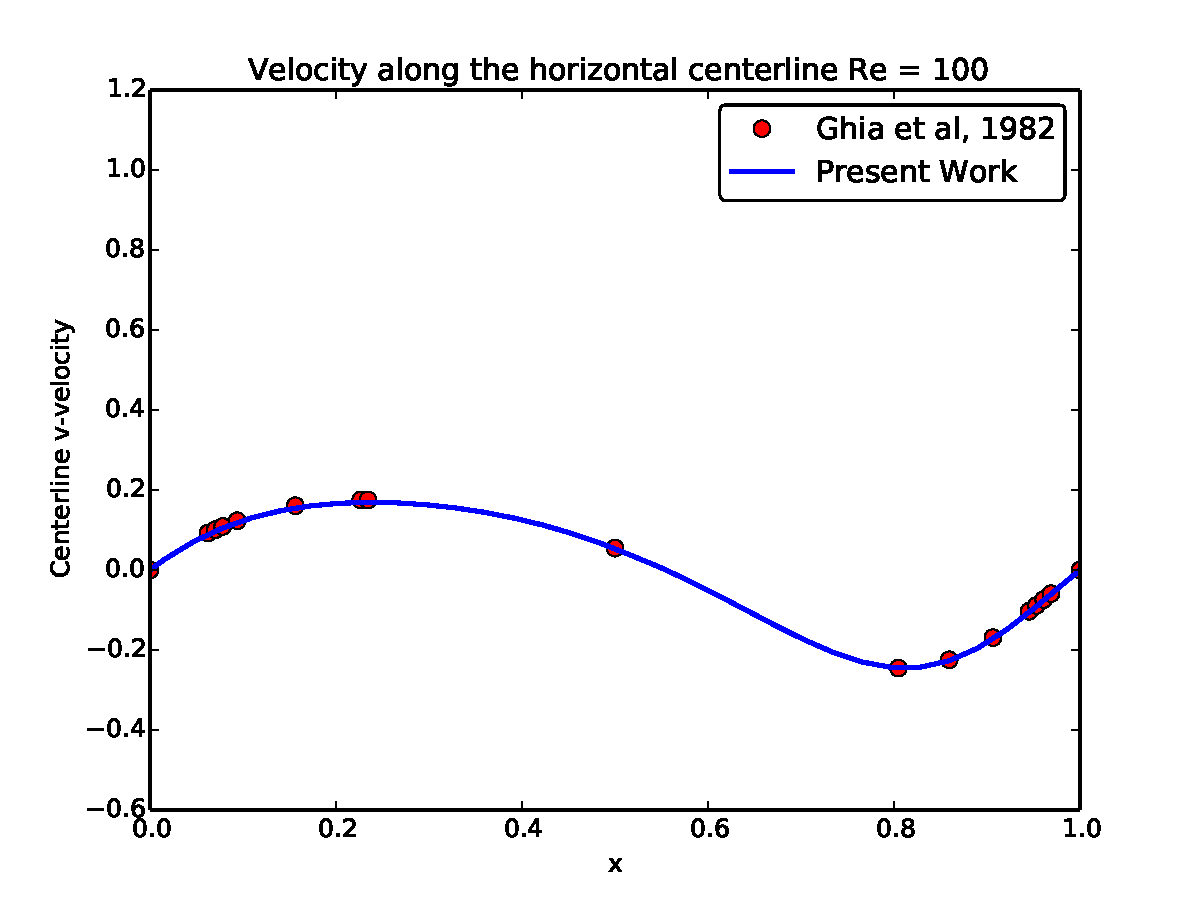
\includegraphics[width=\linewidth]{ldc_horizontal_100}
		\caption{$v$ velocity at the horizontal centerline.}		
	\end{subfigure}
	~
	\begin{subfigure}{0.4\textwidth}
		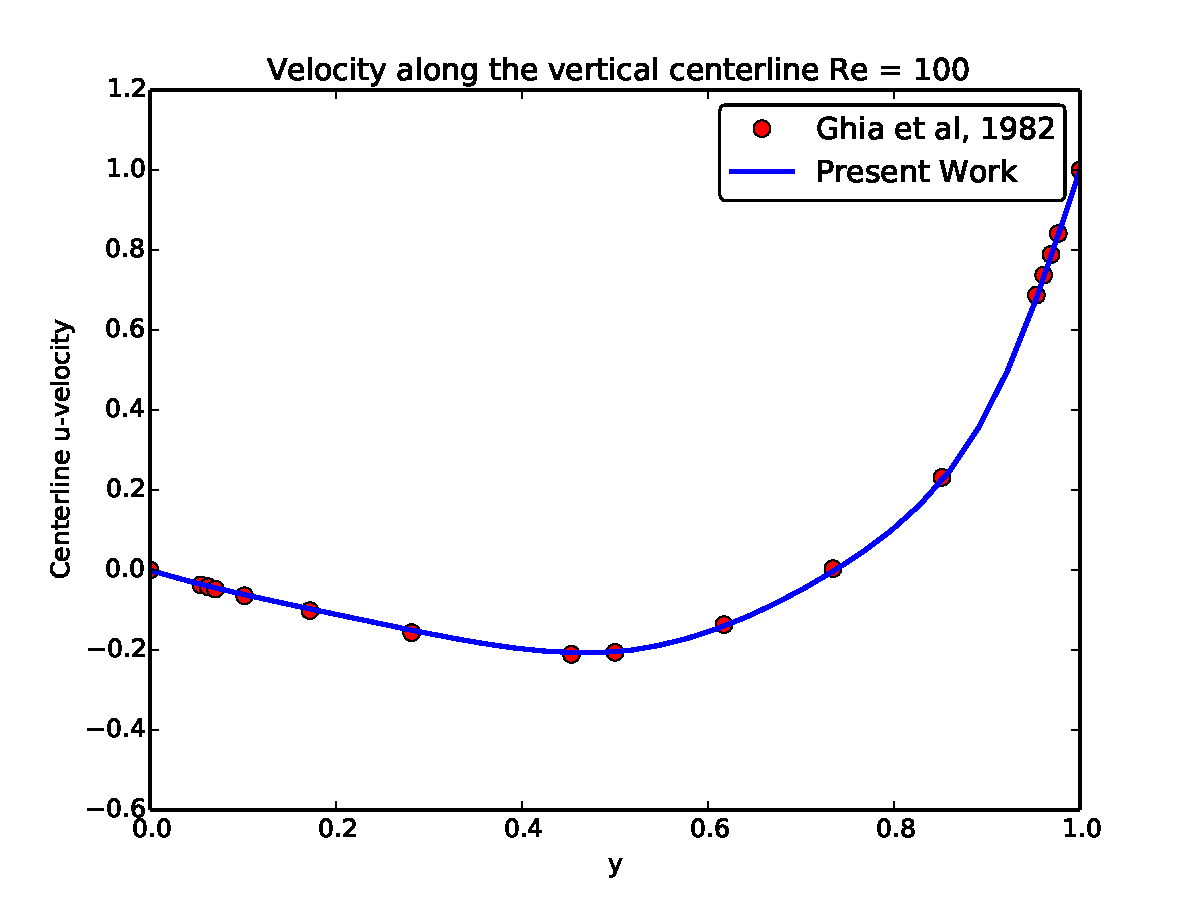
\includegraphics[width=\linewidth]{ldc_vertical_100}
		\caption{$u$ velocity at the vertical centerline.}		
	\end{subfigure}
	\caption{Verification for lid driven cavity with a Reynolds number of 100.}
	\label{fig:ldc100}
\end{figure}

For a Reynolds number of 1000 the domain was discretized into a 128x128 grid. 
What a time step of 0.004 the maximum CFL number works out to be approximately 0.3 using $\Delta t(u/\Delta x+v/\Delta y)$.\todo{find correct cfl number}
In figure \ref{fig:ldc1000} (a) shows the $v$ velocity at the horizontal centerline and (b) shows the $u$ velocity at the vertical centerline. 
\begin{figure}[htb]
	\centering
	\begin{subfigure}{0.4\textwidth}
		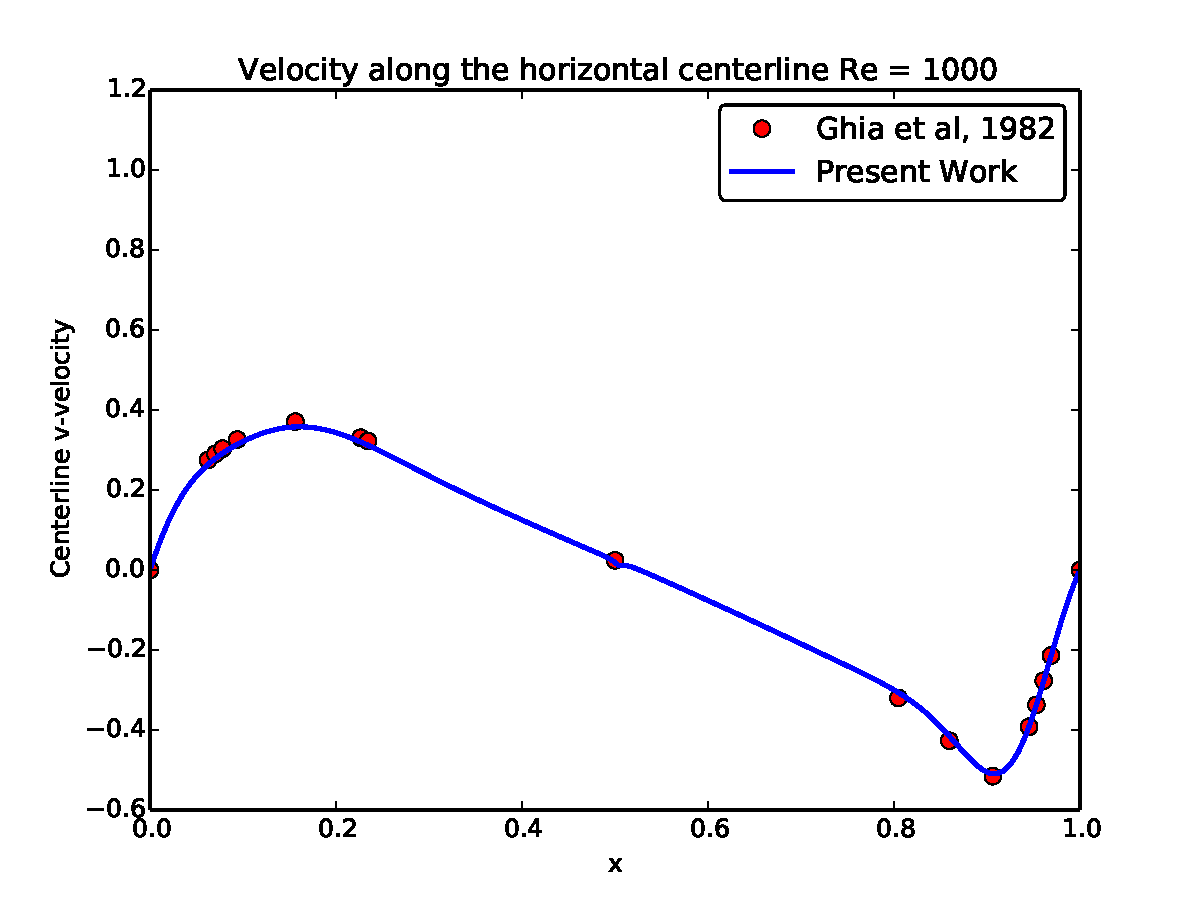
\includegraphics[width=\linewidth]{ldc_horizontal_1000}
		\caption{$v$ velocity at the horizontal centerline.}		
	\end{subfigure}
	~
	\begin{subfigure}{0.4\textwidth}
		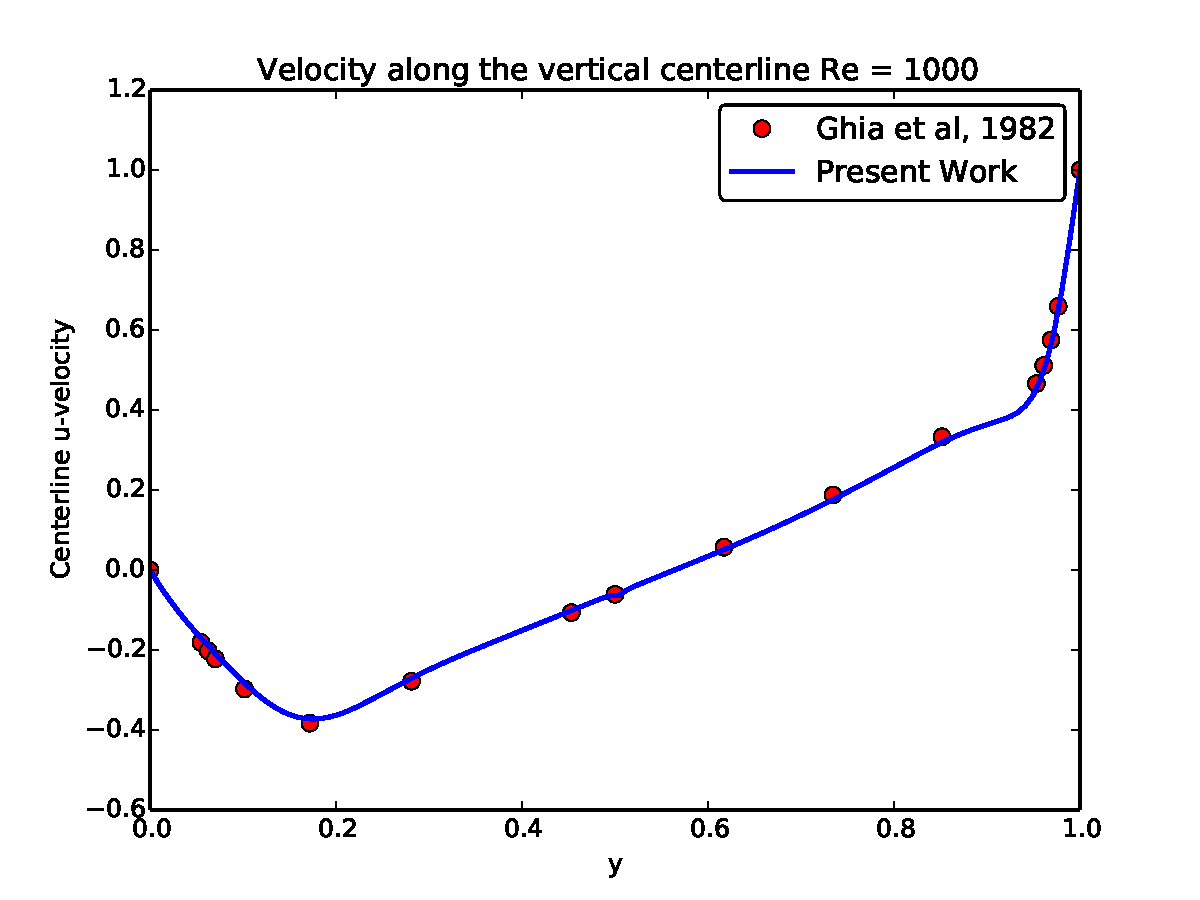
\includegraphics[width=\linewidth]{ldc_vertical_1000}
		\caption{$u$ velocity at the vertical centerline.}		
	\end{subfigure}
	\caption{Verification for lid driven cavity with a Reynolds number of 100.}
	\label{fig:ldc1000}
\end{figure}

\section{Impulsively started cylinder}
The impulsively started cylinder simulation tests the solvers ability to handle an immersed body.
A starting $u$ velocity of one is set in the entire domain.
A Dirichlet inlet, top, and bottom boundaries are set to one as well.
A convective boundary condition is used at the exit.
To verify flow over a stationary cylinder, drag is calculated over time and compared to Koumoutsakos and Leonard~\cite{Koumoutsakos:1995bf}.
Figure \ref{fig:iscylinder} shows the domain of the Reynolds number 40 simulation, the domains for Reynolds number 550 and 3000 have a slightly smaller uniform grid section in the middle.
\begin{figure}[h]
	\centering
	\includestandalone[width=0.5\textwidth]{CylinderDomain}
	\label{fig:iscylinder}
	\caption{The domain of and impulsively started cylinder simulation with Reynolds number forty.}
\end{figure}

All lengths are normalized against the diameter.
For a Reynolds number of 40 a uniform grid with spacing 0.025 is used from (-0.6,-0.6) to (0.6,0.6).
The grid stretches as it moves away from the center until it reaches the domain's edge at $\pm$ 15.
A total of 186x186 cells are used.
\todo{find cfl number}
A time step of 0.005 is used.
Figure \ref{fig:cy40}a and \ref{fig:cy40}b compares the computed drag force of the modified Fadlun et al. and non-embedded Luo et al. methods respectively to that of Koumoutsakos and Leonard.
\begin{figure}[h]
	\centering
	\begin{subfigure}{0.4\textwidth}
		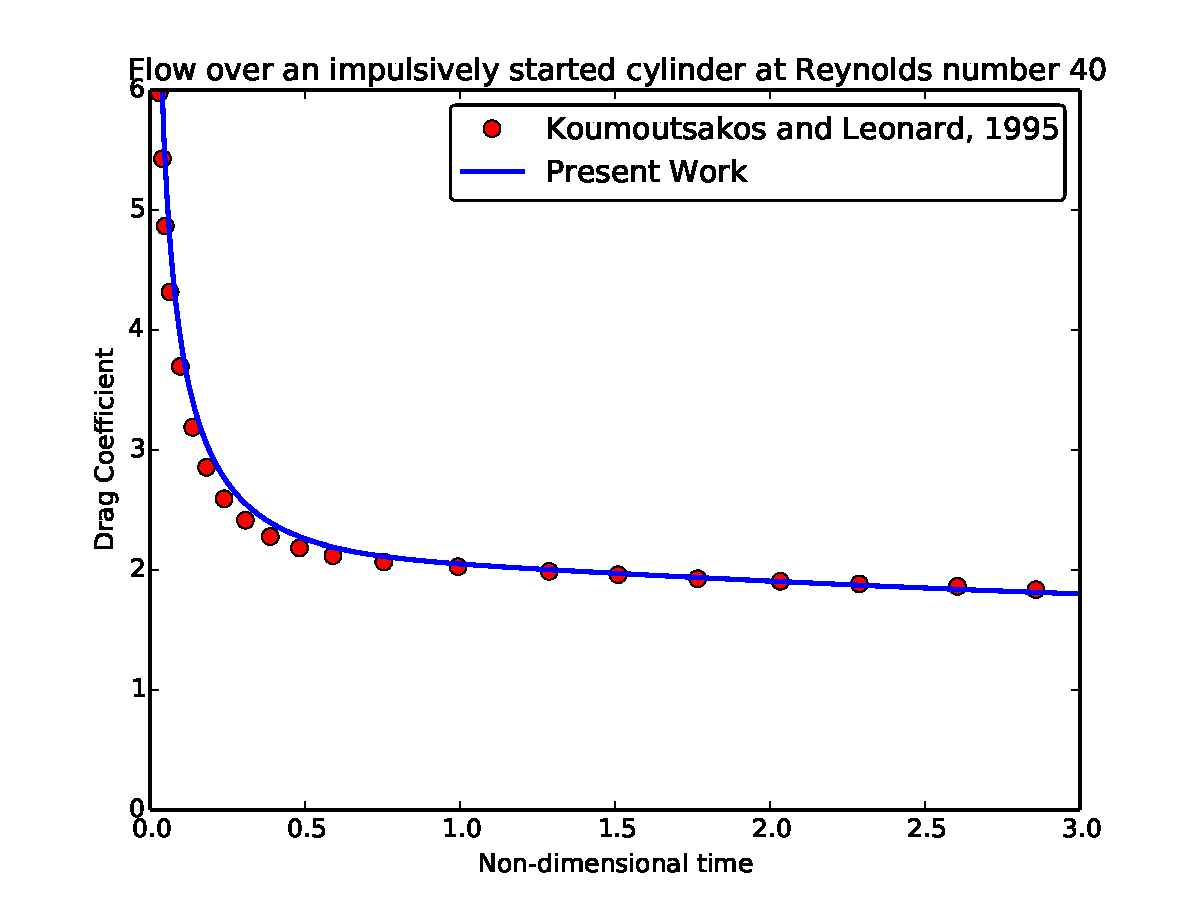
\includegraphics[width=\linewidth]{cy40fadlun}
		\caption{Modified Fadlun et al. style solver.}
	\end{subfigure}
	~
	\begin{subfigure}{0.4\textwidth}
		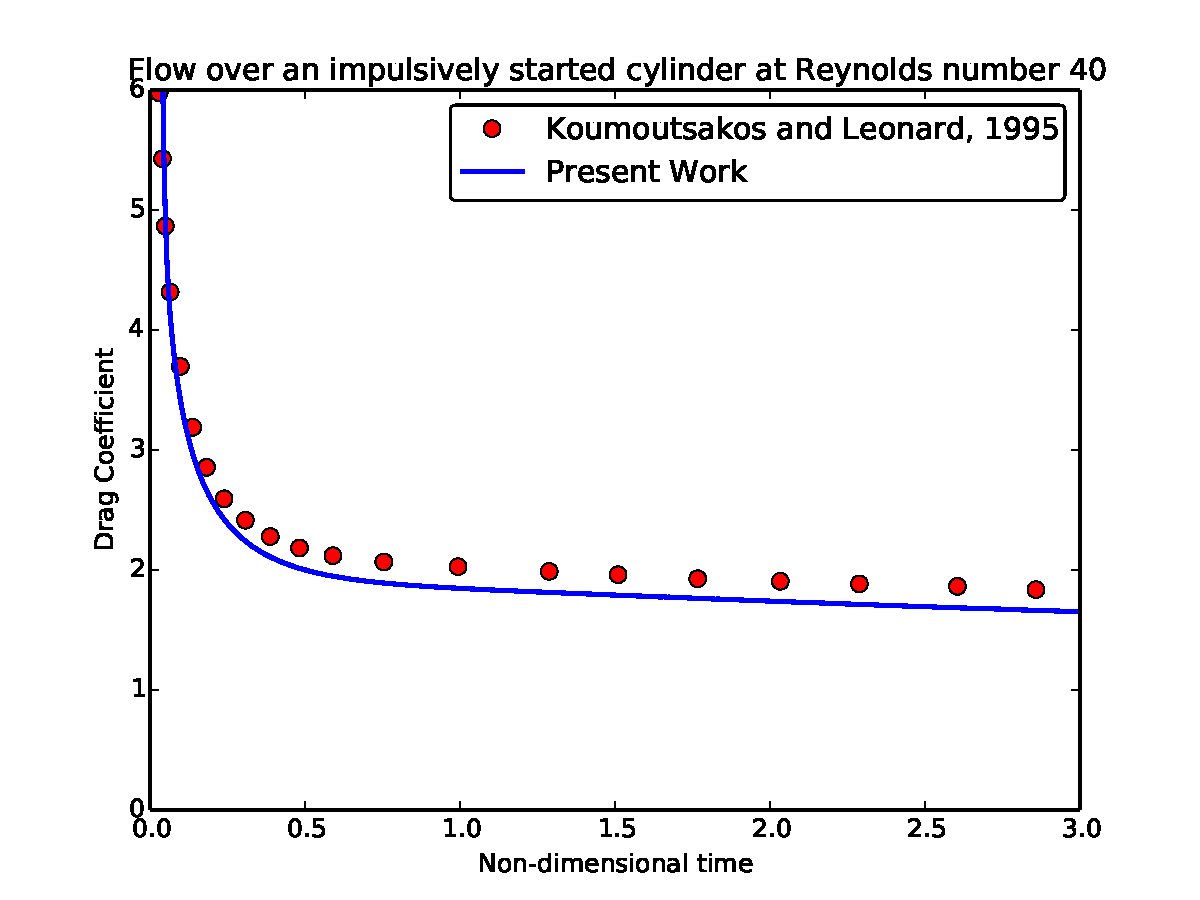
\includegraphics[width=\linewidth]{cy40luo}
		\caption{Non-embedded Luo et al. style solver.}
	\end{subfigure}
	\caption{Drag force verses time for two solvers compared to Koumoutsakos and Leonard for flow over an impulsively started cylinder.}
	\label{fig:cy40}
\end{figure}

For a Reynolds number of 550 a uniform grid with spacing 0.01 is used from (-0.54,-0.54) to (0.54,0.54).
The grid stretches as it moves away from the center until it reaches the domain's edge at $\pm$ 15.
A total of 186x186 cells are used.\todo{update total grid size}
\todo{find cfl number}
A time step of 0.0025 is used.
Figure \ref{fig:cy550}a and \ref{fig:cy550}b compares the computed drag force of the modified Fadlun et al. and non-embedded Luo et al. methods respectively to that of Koumoutsakos and Leonard.
\begin{figure}[h]
	\centering
	\begin{subfigure}{0.4\textwidth}
		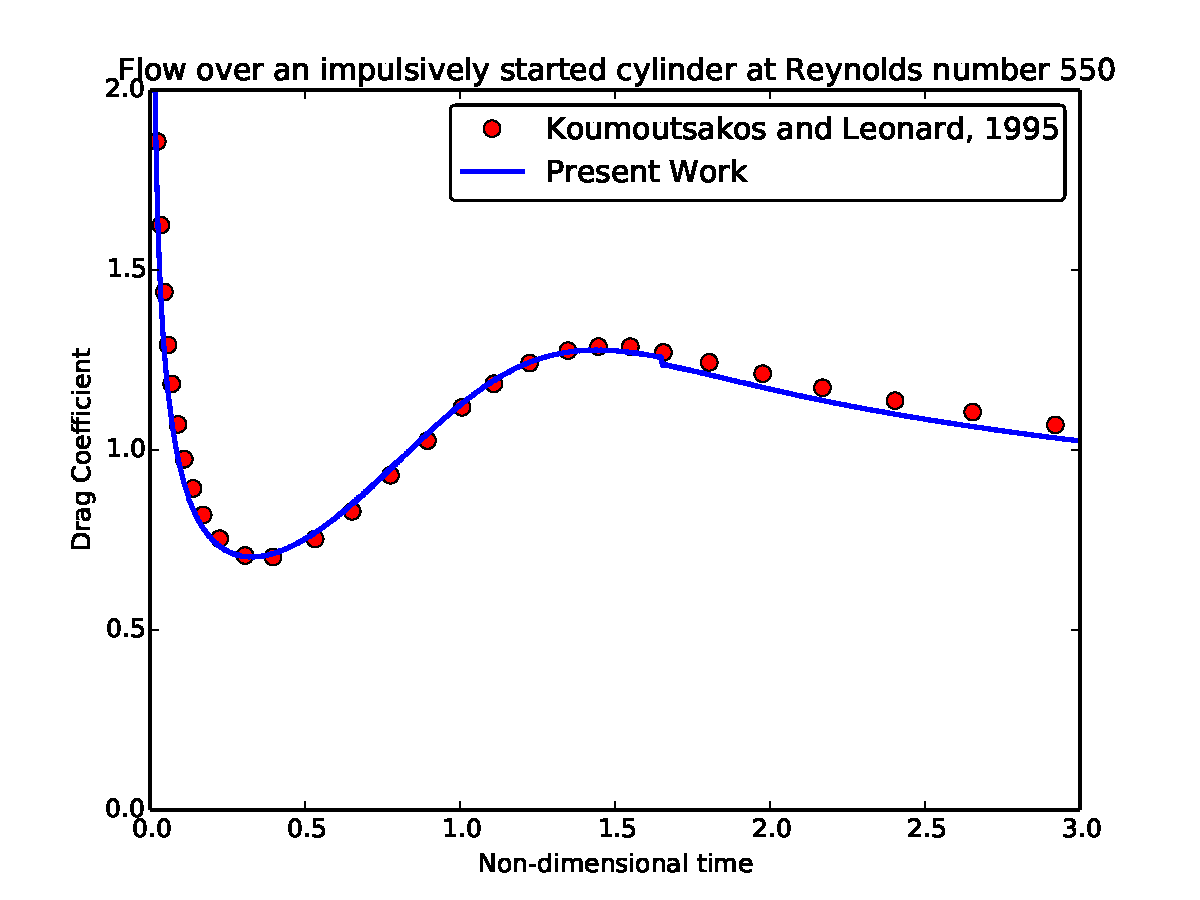
\includegraphics[width=\linewidth]{cy550fadlun}
		\caption{Modified Fadlun et al. style solver.}
	\end{subfigure}
	~
	\begin{subfigure}{0.4\textwidth}
		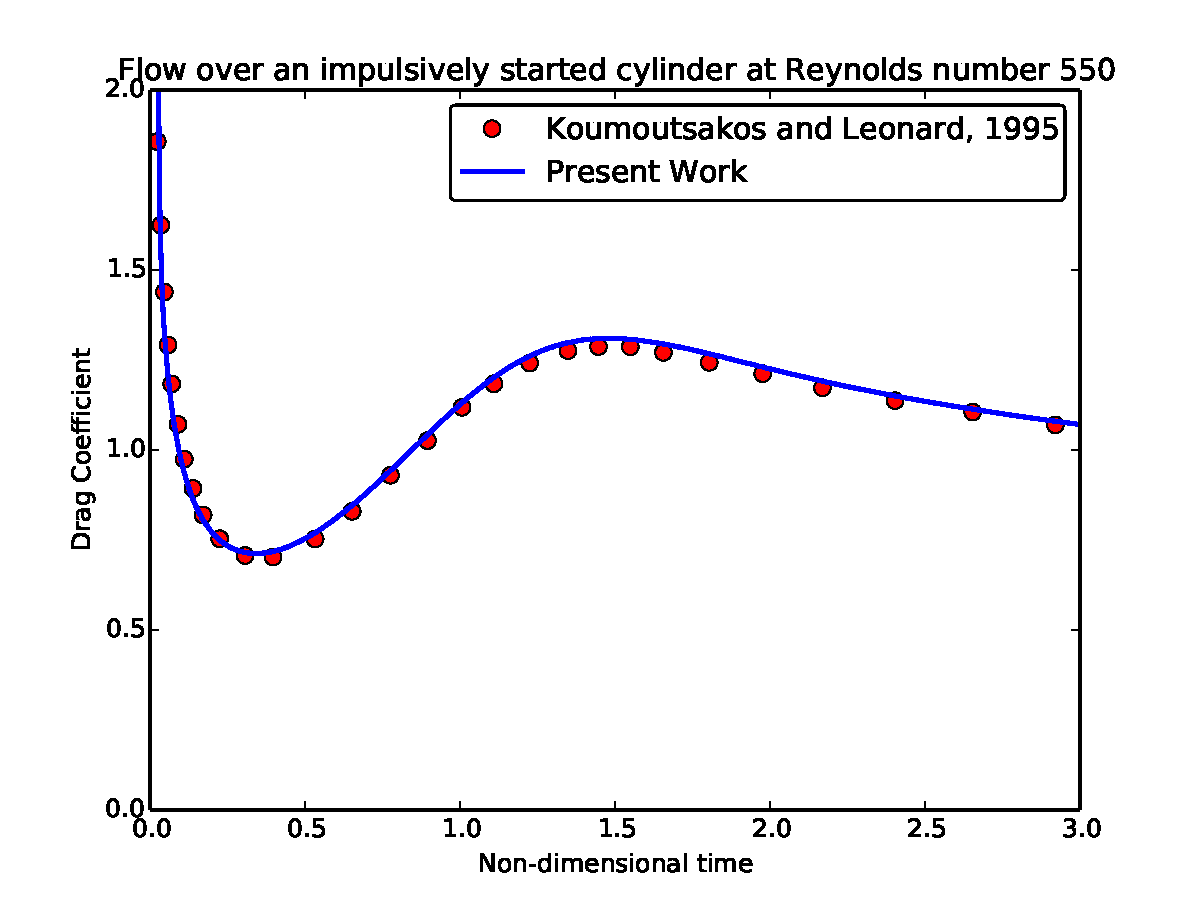
\includegraphics[width=\linewidth]{cy550luo}
		\caption{Non-embedded Luo et al. style solver.}
	\end{subfigure}
	\caption{Drag force verses time for two solvers compared to Koumoutsakos and Leonard for flow over an impulsively started cylinder.}
	\label{fig:cy550}
\end{figure}

All lengths are normalized against the diameter.
For a Reynolds number of 3000 a uniform grid with spacing 0.004 is used from (-0.52,-0.52) to (0.52,0.52).
The grid stretches as it moves away from the center until it reaches the domain's edge at $\pm$ 15.
A total of 186x186 cells are used.\todo{find correct size}
\todo{find cfl number}
A time step of 0.001 is used.
Figure \ref{fig:cy3000}a and \ref{fig:cy3000}b compares the computed drag force of the modified Fadlun et al. and non-embedded Luo et al. methods respectively to that of Koumoutsakos and Leonard.
\begin{figure}[h]
	\centering
	\begin{subfigure}{0.4\textwidth}
		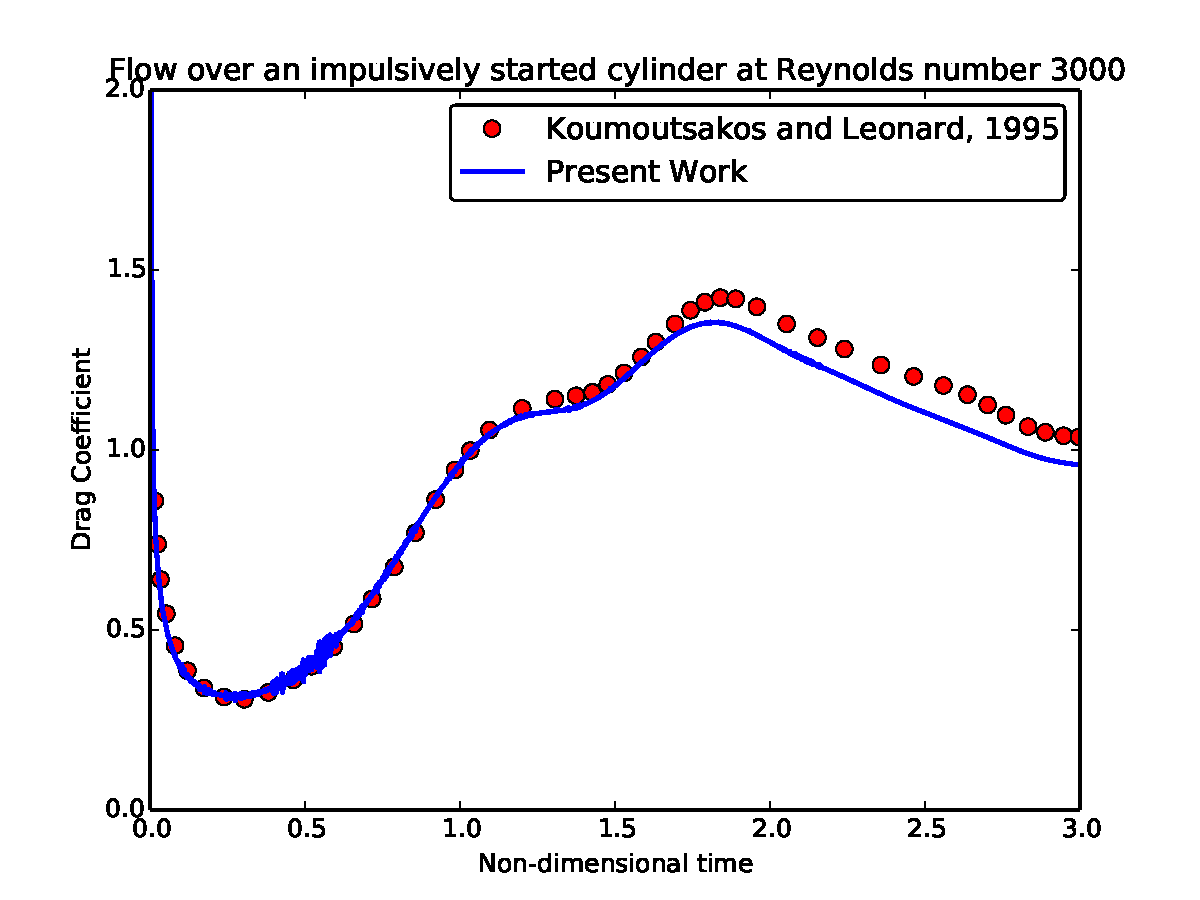
\includegraphics[width=\linewidth]{cy3000fadlun}
		\caption{Modified Fadlun et al. style solver.}
	\end{subfigure}
	~
	\begin{subfigure}{0.4\textwidth}
		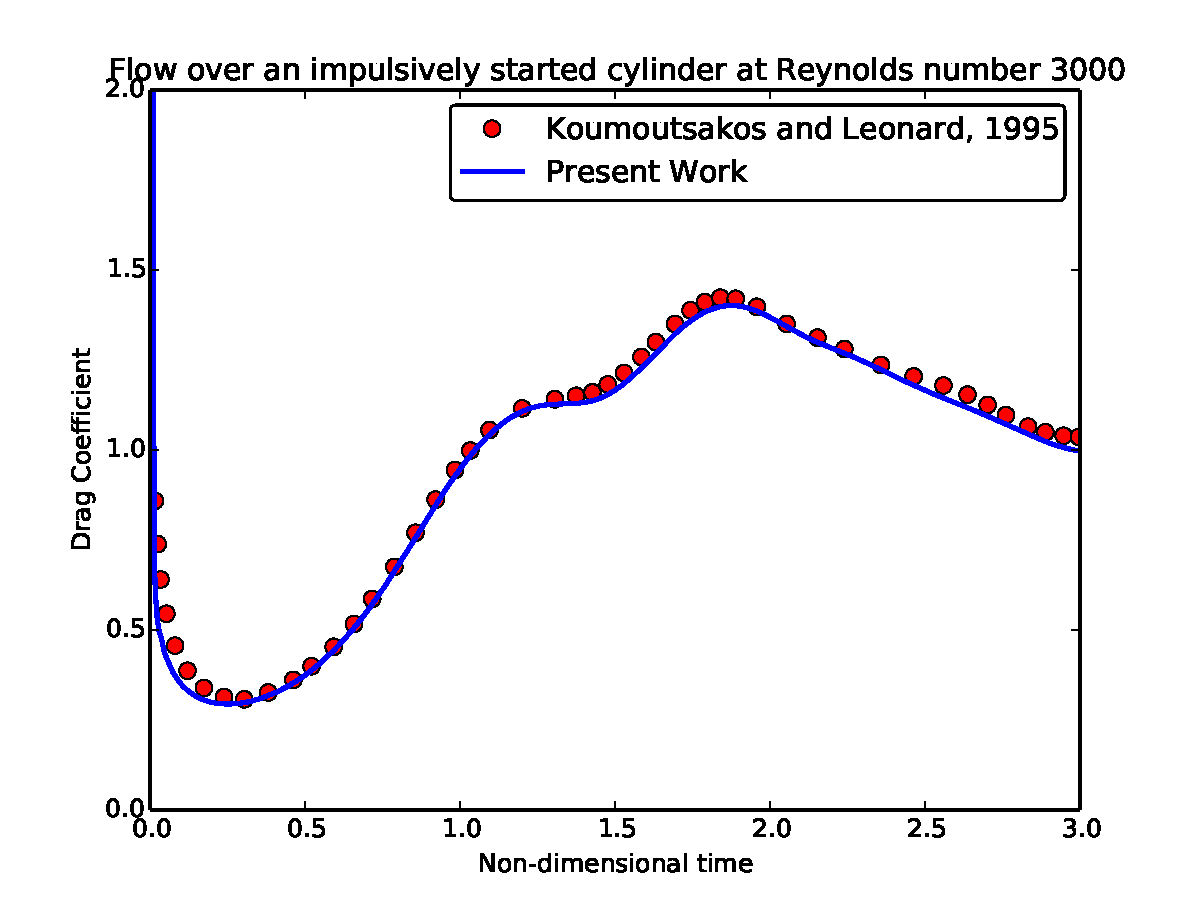
\includegraphics[width=\linewidth]{cy3000luo}
		\caption{Non-embedded Luo et al. style solver.}
	\end{subfigure}
	\caption{Drag force verses time for two solvers compared to Koumoutsakos and Leonard for flow over an impulsively started cylinder.}
	\label{fig:cy3000}
\end{figure}

\section{Impulsively Started Oscillating Cylinder}
The impulsively started oscillating cylinder is a simulation used by Luo et al. to demonstrate a reduction of numerical oscillations between methods.
It is not a verification or validation because it doesn't compare the results to published work, rather it is a useful tool to visualize the numerical oscillations.
A true verification of the moving body is done in the next section,\ref{sec:Oscillating Cylinder in no Flow}
This simulation has the same domain, initial and boundary conditions as the stationary impulsively started cylinder.
The uniform grid at the center spans from (-2,-2) to (2,2) to account for body's movement.

The cylinder moves according to equation \eqref{eq:cylinder position} and \eqref{eq:cylinder velocity}.
The frequency, $f$, is 0.2.
\begin{align}
x&=-0.25\cos{2\pi ft}\label{eq:cylinder position}\\
y&=0.1\pi\sin{2\pi ft}\;\label{eq:cylinder velocity}
\end{align}
Figure \ref{fig:osccylinder} compares the numerical oscillations seen in drag vs time. 
The left column shows drag force experienced the external interpolation and extrapolation Luo et al. style solver.
The right column shows the drag force experience by the embedded interpolation and extrapolation.
The domain for all the simulations ranges from $-15$ to $15$ with a uniform section from $-2$ to $2$.
The uniform section is discretized into a $64 \times 64$ grid for the first row and $ 128 \times 128$ grid for last three rows row.
The maximum CFL numbers by row are approximately \numlist{0.35; 0.35; 0.7; 1.0}.
\begin{figure}[h]
	\centering
	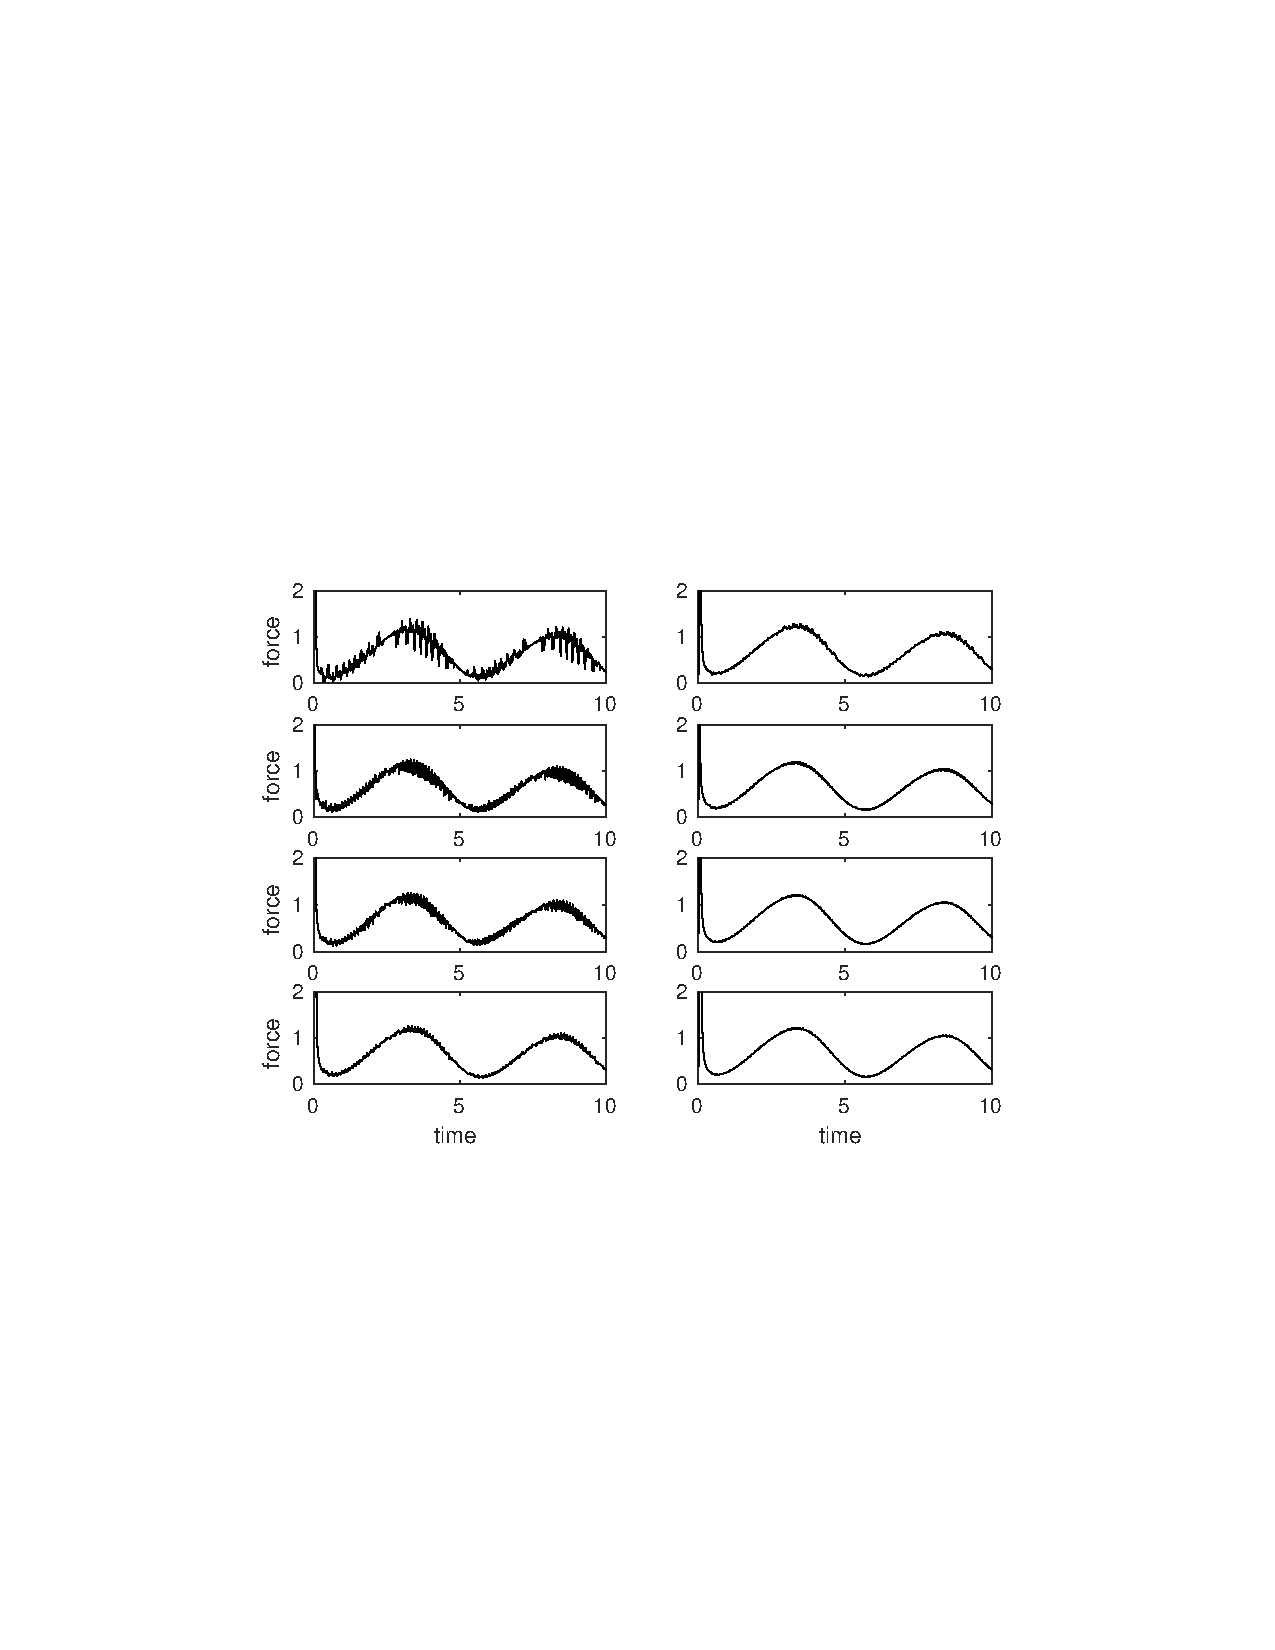
\includegraphics[width=\textwidth]{cropped_oscflow}
	\caption{The left column shows external interpolation and the right column shows the embedded interpolation. Rows one though four are maximum CFL \numlist{0.35; 0.35; 0.7; 1.0} and have a middle grid spacing of \numlist{0.0625; 0.03125; 0.03125; 0.03125}}
	\label{fig:osccylinder}
\end{figure}\todo{fix time label on 3rd row}


\section{Oscillating Cylinder in no Flow}
\label{sec:Oscillating Cylinder in no Flow}
The oscillation of a cylinder in no flow is verified against the work of Liao et al. \cite{liao2010simulating}. 
The equations that govern movement,\ref{eq:cylinder position2} and \ref{eq:cylinder velocity2} are the same form as above with different coefficients.
The domain is also the same as the impulsively started oscillating cylinder.
Frequency is set at one.
\begin{align}
x&=\frac{-1}{2\pi}\sin{2\pi ft}\label{eq:cylinder position2}\\
y&=-cos{2\pi ft}\;\label{eq:cylinder velocity2}
\end{align}

Figure \ref{fig:staticInit}shows the drag during the first period versus the steady state drag from Liao et al.
Figure \ref{fig:static2} shows the drag during the second period.
In both figures, (a) is external interpolation and (b) is embedded interpolation.
 
\begin{figure}[h]
	\centering
	\begin{subfigure}{0.4\textwidth}
		\includegraphics[width=\linewidth]{staticInitLuo}
		\caption{External interpolation method.}
	\end{subfigure}
	~
	\begin{subfigure}{0.4\textwidth}
		\includegraphics[width=\linewidth]{staticInitOsc}
		\caption{Embedded interpolation method.}
	\end{subfigure}
	\caption{Drag force verses time for the first period compared to steady state Liao et al. for an oscillating cylinder in no flow.}
	\label{fig:staticInit}
\end{figure}

\begin{figure}[h]
	\centering
	\begin{subfigure}{0.4\textwidth}
		\includegraphics[width=\linewidth]{static2Luo}
		\caption{External interpolation method.}
	\end{subfigure}
	~
	\begin{subfigure}{0.4\textwidth}
		\includegraphics[width=\linewidth]{static2Osc}
		\caption{Embedded interpolation method.}
	\end{subfigure}
	\caption{Drag force verses time for steady state oscillating cylinder in now flow compared to Liao et al.}
	\label{fig:static2}
\end{figure}
\todo{change referecne to DUTSCH et al experimental data}

\section{Vorticity Induced Vibration}
The vorticity induced vibration simulation tests the solvers ability to predict the position of a freely moving body in coupled fluid structure interaction.
The domain is the same as the impulsively started cylinder simulation except the uniform region ranges from -1 to 1 and -1.5 to 1.5 in the x and y respectively.
An immersed cylinder starts at the origin with no initial velocity.
The body is free to move in the y direction but fixed in the x and is mounted to a spring to prevent it from wandering off.
In VIV the Reynolds number is set in a range that sheds oscillating vortices.
This combined with the spring causes the body to establish a steady state sinusoidal motion for which the amplitude can be verified.
Following the work of Borazjani et al. the mass spring damper system \eqref{eq:masspring} that governs the body's movement is non-dimensionalized to become equation \eqref{eq:ndmasspring}.
\begin{equation}
M\frac{\partial^2Y}{\partial t^2}+C\frac{\partial Y}{\partial t}+KY=F_y \label{eq:masspring}
\end{equation}
$Y$ is the center coordinate of the body, $M$ is the mass, $C$ is the damping factor, $K$ is the stiffness and $F_y$ is the total fluid force on the body in the y direction. 
The natural frequency and critical damping are given by \eqref{eq:nf} and \eqref{eq:cd}.
\begin{align}
\omega &=2\pi f =\sqrt{\frac{K}{M}}\label{eq:nf}\\
C_{cr}&=2\sqrt{MK}=2K\omega \; \label{eq:cd}
\end{align}
\begin{equation}
\frac{\partial^2 Y}{\partial t^2}+4\pi \zeta\frac{1}{U_{red}}\frac{\partial Y}{\partial t}+4\pi^2\frac{1}{u_{red}^2}Y=\frac{1}{2M_{red}}C_Y\label{eq:ndmasspring}
\end{equation}
Borazjani et al. defines the non-dimensional coefficients as follows:

Damping coefficient
\begin{equation}
\zeta=\frac{C}{C_{cr}}\label{eq:damping coefficient}
\end{equation}
Reduced velocity
\begin{equation}
U_{red}=\frac{U}{fD}\label{eq:reduced velocity}
\end{equation}
Reduced mass
\begin{equation}
M_{red}=\frac{M}{\rho D^2}\label{eq:reduced mass}
\end{equation}
Force coefficient
\begin{equation}
C_Y=\frac{2F_Y}{\rho U^2 D}\label{eq:force coefficient}
\end{equation}
In this simulation, Re is set to 150, $\zeta$ is set to 0, $M_red$ is set to 2 and $U_{red}$ is varied between 3 and 8.

There are two different ways to update body position, loose and strong coupling.
Loose coupling comes from the explicit derivation of equation \eqref{eq:ndmasspring}.
A time step using loose coupling looks as follows:
\begin{enumerate}
	\item Solve for field values at $t^{n+1}$ using Naiver--Stokes.
	\item Calculate body forces.
	\item Move body using equations \eqref{eq:lc1} and \eqref{eq:lc2}.
\end{enumerate}
\begin{align}
v^{n+1} &= v^n-\frac{dt\pi^24}{U_{red}^2}\left(y^n+\frac{dtv^n}{2}\right) + \frac{dtC_Y}{\left(2M_{red}\right)\left(1+\frac{4dt^2\pi^2}{U_{red}^2}\right)} \label{eq:lc1} \\
y^{n+1} &= y^n +\frac{dt\left(v^{n+1}+v^n\right)}{2}\; \label{eq:lc2}
\end{align}

Equation \eqref{eq:ndmasspring} can also be discretized implicitly.
This is know as strong coupling.
A strong coupling time step repeatly calculates the new body position is converged on:
\begin{enumerate}
	\item Solve for field values at sub step $t^{k+1}$ using Naiver--Stokes.
	\item Calculate body forces
	\item Move body using equations \eqref{eq:lc1} and \eqref{eq:sc}.
	\item If $|Y^{k+1}-Y^k| \approx 0$ advance time, otherwise advance sub step.
\end{enumerate}
\begin{equation}
y^{k+1} = \alpha \left(y^n+\frac{dt\left(v^{k+1}+v^n\right)}{2}\right) +\left(1-\alpha\right)y^k\label{eq:sc}
\end{equation}

Figures \ref{fig:viv1}, \ref{fig:viv2}, \ref{fig:viv3} and \ref{fig:viv4} show the maximum amplitude of the 6 VIV simulations as calculated by loose coupling external interpolation, strong coupling external interpolation, loose coupling embedded interpolation and strong coupling embedded interpolation respectively.
Results are verified against the curvilinear immeresed boundary method of Borazjani et al.\cite{borazjani2008curvilinear} and the unstructured finite-element ALE approach of Ahn and Kallinderis\cite{ahn2006strongly}.
\begin{figure}
	\centering
	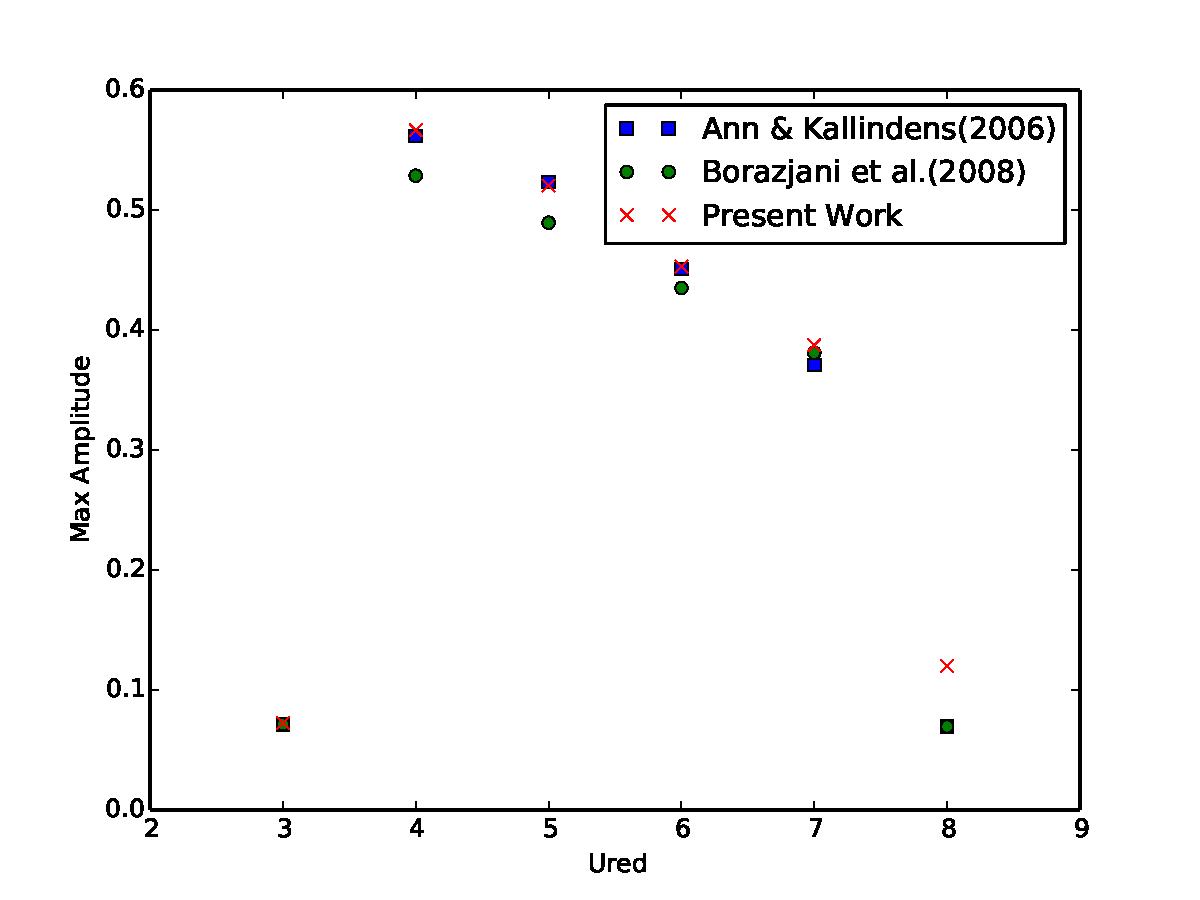
\includegraphics[width=\textwidth]{vivexlc}
	\caption{The maximum amplitude vs reduced velocity for the VIV lock in region calculated with external interpolation and loose coupling.}
	\label{fig:viv1}
\end{figure}
\begin{figure}
	\centering
	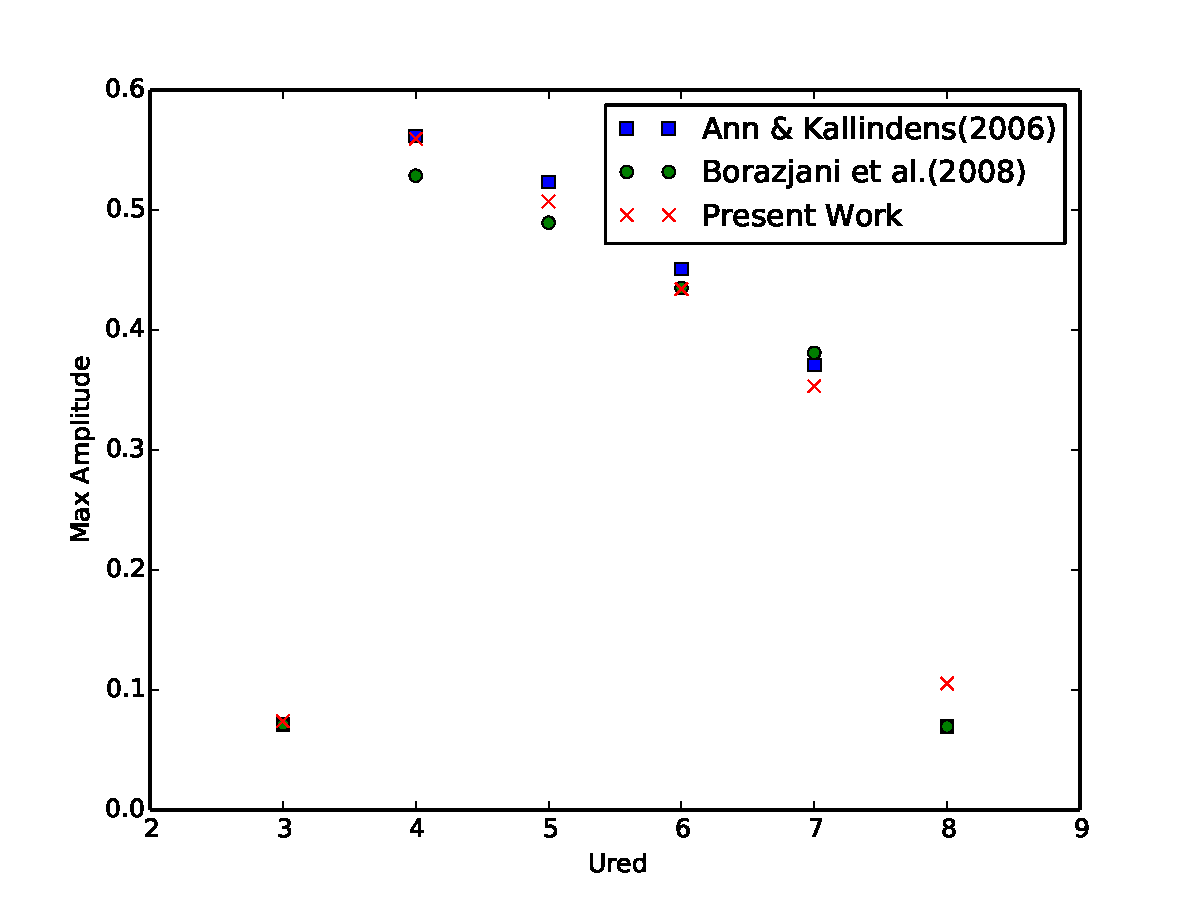
\includegraphics[width=\textwidth]{vivexsc}
	\caption{The maximum amplitude vs reduced velocity for the VIV lock in region calculated with external interpolation and strong coupling.}
	\label{fig:viv2}
\end{figure}
\begin{figure}
	\centering
	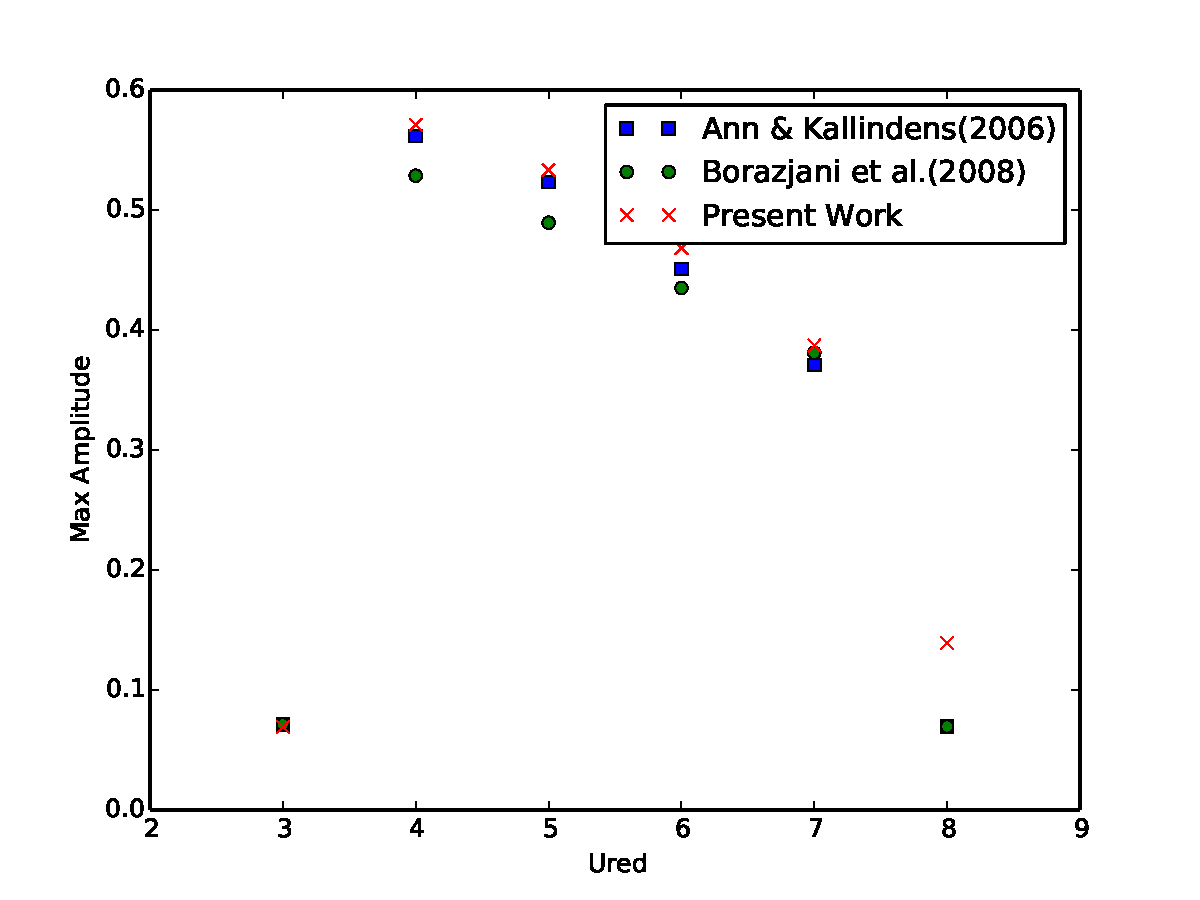
\includegraphics[width=\textwidth]{vivemlc}
	\caption{The maximum amplitude vs reduced velocity for the VIV lock in region calculated with embedded interpolation and loose coupling.}
	\label{fig:viv3}
\end{figure}
\begin{figure}
	\centering
	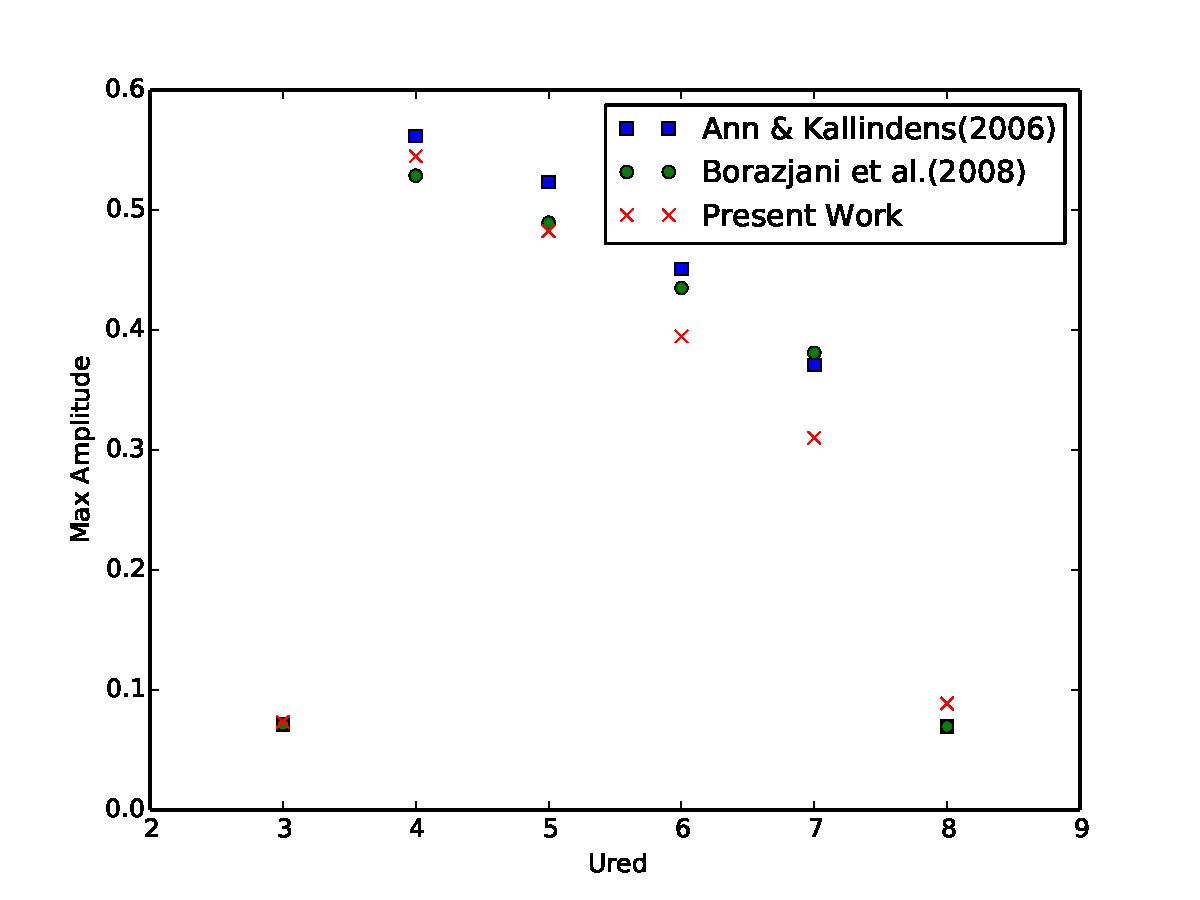
\includegraphics[width=\textwidth]{vivemsc}
	\caption{The maximum amplitude vs reduced velocity for the VIV lock in region calculated with embedded interpolation and strong coupling.}
	\label{fig:viv4}
\end{figure}

\chapter{Conclusions}
\section{Error Analysis}


\subsection{Modified Fadlun}
Cylinder
osc cylinder
viv
\subsection{Embedded Luo}
Cylinder
osc cylinder
viv
	LC
	SC
\subsection{External Luo}
Cylinder
osc cylinder
viv
	LC
	SC

\section{Performance Scaling}

\chapter{Future Work}

\bibliographystyle{plain}
\bibliography{thesis}

\appendix
\chapter{Discretization}
\section{Fadlun}
\subsection{Fadlun Linear Interpolation}\label{Fadlun Linear Interpolation}
\section{Luo}
\subsection{Solving a system of four eqations on the gpu}\label{system of euqations}
\subsection{a: interpolation to hybrid nodes}
\label{a: interpolation to hybrid nodes}

\end{document}
